% Generated by Sphinx.
\documentclass[letterpaper,10pt,english]{manual}
\usepackage[utf8]{inputenc}
\usepackage[T1]{fontenc}
\usepackage{babel}
\usepackage{times}
\usepackage[Bjarne]{fncychap}
\usepackage{longtable}
\usepackage{sphinx}


\title{TortoiseHg Documentation}
\date{March 05, 2010}
\release{1.0.0}
\author{Steve Borho and others}
\newcommand{\sphinxlogo}{
\includegraphics{thg_logo_pdf.png}\par}
\renewcommand{\releasename}{Release}
\makeindex
\makemodindex
\newcommand\PYGZat{@}
\newcommand\PYGZlb{[}
\newcommand\PYGZrb{]}
\newcommand\PYGaz[1]{\textcolor[rgb]{0.00,0.63,0.00}{#1}}
\newcommand\PYGax[1]{\textcolor[rgb]{0.84,0.33,0.22}{\textbf{#1}}}
\newcommand\PYGay[1]{\textcolor[rgb]{0.00,0.44,0.13}{\textbf{#1}}}
\newcommand\PYGar[1]{\textcolor[rgb]{0.73,0.38,0.84}{#1}}
\newcommand\PYGas[1]{\textcolor[rgb]{0.25,0.44,0.63}{\textit{#1}}}
\newcommand\PYGap[1]{\textcolor[rgb]{0.00,0.44,0.13}{\textbf{#1}}}
\newcommand\PYGaq[1]{\textcolor[rgb]{0.38,0.68,0.84}{#1}}
\newcommand\PYGav[1]{\textcolor[rgb]{0.00,0.44,0.13}{\textbf{#1}}}
\newcommand\PYGaw[1]{\textcolor[rgb]{0.13,0.50,0.31}{#1}}
\newcommand\PYGat[1]{\textcolor[rgb]{0.73,0.38,0.84}{#1}}
\newcommand\PYGau[1]{\textcolor[rgb]{0.32,0.47,0.09}{#1}}
\newcommand\PYGaj[1]{\textcolor[rgb]{0.00,0.44,0.13}{#1}}
\newcommand\PYGak[1]{\textcolor[rgb]{0.14,0.33,0.53}{#1}}
\newcommand\PYGah[1]{\textcolor[rgb]{0.00,0.13,0.44}{\textbf{#1}}}
\newcommand\PYGai[1]{\textcolor[rgb]{0.73,0.38,0.84}{#1}}
\newcommand\PYGan[1]{\textcolor[rgb]{0.13,0.50,0.31}{#1}}
\newcommand\PYGao[1]{\textcolor[rgb]{0.25,0.44,0.63}{\textbf{#1}}}
\newcommand\PYGal[1]{\textcolor[rgb]{0.00,0.44,0.13}{\textbf{#1}}}
\newcommand\PYGam[1]{\textbf{#1}}
\newcommand\PYGab[1]{\textit{#1}}
\newcommand\PYGac[1]{\textcolor[rgb]{0.25,0.44,0.63}{#1}}
\newcommand\PYGaa[1]{\textcolor[rgb]{0.19,0.19,0.19}{#1}}
\newcommand\PYGaf[1]{\textcolor[rgb]{0.25,0.50,0.56}{\textit{#1}}}
\newcommand\PYGag[1]{\textcolor[rgb]{0.13,0.50,0.31}{#1}}
\newcommand\PYGad[1]{\textcolor[rgb]{0.00,0.25,0.82}{#1}}
\newcommand\PYGae[1]{\textcolor[rgb]{0.13,0.50,0.31}{#1}}
\newcommand\PYGaZ[1]{\textcolor[rgb]{0.25,0.44,0.63}{#1}}
\newcommand\PYGbf[1]{\textcolor[rgb]{0.00,0.44,0.13}{#1}}
\newcommand\PYGaX[1]{\textcolor[rgb]{0.25,0.44,0.63}{#1}}
\newcommand\PYGaY[1]{\textcolor[rgb]{0.00,0.44,0.13}{#1}}
\newcommand\PYGbc[1]{\textcolor[rgb]{0.78,0.36,0.04}{#1}}
\newcommand\PYGbb[1]{\textcolor[rgb]{0.00,0.00,0.50}{\textbf{#1}}}
\newcommand\PYGba[1]{\textcolor[rgb]{0.02,0.16,0.45}{\textbf{#1}}}
\newcommand\PYGaR[1]{\textcolor[rgb]{0.25,0.44,0.63}{#1}}
\newcommand\PYGaS[1]{\textcolor[rgb]{0.13,0.50,0.31}{#1}}
\newcommand\PYGaP[1]{\textcolor[rgb]{0.05,0.52,0.71}{\textbf{#1}}}
\newcommand\PYGaQ[1]{\textcolor[rgb]{0.78,0.36,0.04}{\textbf{#1}}}
\newcommand\PYGaV[1]{\textcolor[rgb]{0.25,0.50,0.56}{\textit{#1}}}
\newcommand\PYGaW[1]{\textcolor[rgb]{0.05,0.52,0.71}{\textbf{#1}}}
\newcommand\PYGaT[1]{\textcolor[rgb]{0.73,0.38,0.84}{#1}}
\newcommand\PYGaU[1]{\textcolor[rgb]{0.13,0.50,0.31}{#1}}
\newcommand\PYGaJ[1]{\textcolor[rgb]{0.56,0.13,0.00}{#1}}
\newcommand\PYGaK[1]{\textcolor[rgb]{0.25,0.44,0.63}{#1}}
\newcommand\PYGaH[1]{\textcolor[rgb]{0.50,0.00,0.50}{\textbf{#1}}}
\newcommand\PYGaI[1]{\fcolorbox[rgb]{1.00,0.00,0.00}{1,1,1}{#1}}
\newcommand\PYGaN[1]{\textcolor[rgb]{0.73,0.73,0.73}{#1}}
\newcommand\PYGaO[1]{\textcolor[rgb]{0.00,0.44,0.13}{#1}}
\newcommand\PYGaL[1]{\textcolor[rgb]{0.02,0.16,0.49}{#1}}
\newcommand\PYGaM[1]{\colorbox[rgb]{1.00,0.94,0.94}{\textcolor[rgb]{0.25,0.50,0.56}{#1}}}
\newcommand\PYGaB[1]{\textcolor[rgb]{0.25,0.44,0.63}{#1}}
\newcommand\PYGaC[1]{\textcolor[rgb]{0.33,0.33,0.33}{\textbf{#1}}}
\newcommand\PYGaA[1]{\textcolor[rgb]{0.00,0.44,0.13}{#1}}
\newcommand\PYGaF[1]{\textcolor[rgb]{0.63,0.00,0.00}{#1}}
\newcommand\PYGaG[1]{\textcolor[rgb]{1.00,0.00,0.00}{#1}}
\newcommand\PYGaD[1]{\textcolor[rgb]{0.00,0.44,0.13}{\textbf{#1}}}
\newcommand\PYGaE[1]{\textcolor[rgb]{0.25,0.50,0.56}{\textit{#1}}}
\newcommand\PYGbg[1]{\textcolor[rgb]{0.44,0.63,0.82}{\textit{#1}}}
\newcommand\PYGbe[1]{\textcolor[rgb]{0.40,0.40,0.40}{#1}}
\newcommand\PYGbd[1]{\textcolor[rgb]{0.25,0.44,0.63}{#1}}
\newcommand\PYGbh[1]{\textcolor[rgb]{0.00,0.44,0.13}{\textbf{#1}}}
\begin{document}

\maketitle
\tableofcontents



Contents:

\resetcurrentobjects
\hypertarget{--doc-preface}{}

\chapter{Preface}
\index{preface (module)}
\hypertarget{module-preface}{}
\declaremodule[preface]{}{preface}
\modulesynopsis{About this manual}

\section{Audience}

This book is written for computer literate folk who want to use
Mercurial to manage their data, but are uncomfortable using the command
line client to do so. Since TortoiseHg is a Windows shell extension it's
assumed that the user is familiar with the Windows explorer and knows
how to use it.

You can find the most up to date version of this documentation at our
\href{http://tortoisehg.org}{web} site.


\section{Reading guide}

This Preface explains a little about the TortoiseHg project, the
community of people who work on it, and the licensing conditions for
using it and distributing it.

The \hyperlink{--doc-intro}{\emph{Introduction}} explains what TortoiseHg is, what it does, where it
comes from and the basics for installing it on your PC.

\hyperlink{--doc-quick}{\emph{A Quick Start Guide to TortoiseHg}} is a quick tutorial on how to start with TortoiseHg.

\hyperlink{--doc-daily}{\emph{TortoiseHg in daily use}} is the main chapter, it describes the frequently used
components of TortoiseHg.

\hyperlink{--doc-settings}{\emph{Settings}} describes how to configure TortoiseHg.

\hyperlink{--doc-recovery}{\emph{Recovery}} describes the recovery operations one can perform on a
project.

\hyperlink{--doc-nonhg}{\emph{Use with other VCS systems}} describes how to use TortoiseHg as a client to
non-Mercurial servers.

\hyperlink{--doc-faq}{\emph{Frequently Asked Questions}} has a list of common questions and their answers.

\hyperlink{--doc-debugging}{\emph{Debugging}} describes how to debug any problems that you find.


\section{TortoiseHg is free!}

TortoiseHg is released under
\href{http://www.gnu.org/licenses/gpl-2.0.html}{GPLv2}.  You are free to
install it on as many computers as you like, and to redistribute it
according to the GPLv2 license.


\section{Community}

Mailing Lists:
\begin{itemize}
\item {} 
\href{https://lists.sourceforge.net/lists/listinfo/tortoisehg-discuss}{Users} - Announcements, user Q\&A, and feature discussions.

\item {} 
\href{https://lists.sourceforge.net/lists/listinfo/tortoisehg-develop}{Developers} - Patches, bug reports, development discussions.

\item {} 
\href{https://lists.sourceforge.net/lists/listinfo/tortoisehg-issues}{Issues} - Notifications from the issue tracker.

\end{itemize}

And our \href{http://bitbucket.org/tortoisehg/stable/wiki/Home}{wiki} on Bitbucket.


\section{Acknowledgement}

Thanks to the many people who contribute to the TortoiseHg project.  It
takes a community of developers, translators, and users to build a
truly useful tool.  Especially users who care enough to report bugs and
file feature requests.

The TortoiseHg installer for Windows includes the TortoiseOverlays handler,
as provided by the \href{http://tortoisesvn.net}{TortoiseSVN} project.


\section{Conventions used in this manual}

The following typographical conventions are used in this manual:
\begin{description}
\item[\code{Ctrl-A}]
Indicates a key, or combination of keys, to press.

\item[\textbf{Commit}]
Indicates a label, button or anything that appears in user interfaces.

\item[\emph{TortoiseHg... \(\rightarrow\) About}]
Indicates a menu choice, or a combination of menu choice, tab
selection and GUI label.  For example
\emph{TortoiseHg...  \(\rightarrow\) Global settings \(\rightarrow\) Commit \(\rightarrow\) User name}
means do something in \textbf{User name} label under
\textbf{Commit} tab selectable from the menu choice
\emph{TortoiseHg... \(\rightarrow\) Global settings}.

\item[\code{.hg/hgrc}]
Indicates a filename or directory name.

\item[\textbf{hgtk log}]
Indicates a command to enter into command window.

\item[\code{myproxy:8000}]
Indicates a text to enter into a text input field in the GUI.

\end{description}

\begin{notice}{note}{Note:}
This is a note.
\end{notice}

\begin{notice}{warning}{Warning:}
An important note. Pay attention.
\end{notice}

\resetcurrentobjects
\hypertarget{--doc-intro}{}

\chapter{Introduction}
\index{introduction (module)}
\hypertarget{module-introduction}{}
\declaremodule[introduction]{}{introduction}
\modulesynopsis{Introduce TortoiseHg and its various parts}

\section{What is TortoiseHg?}

TortoiseHg is a set of graphical tools and a shell extension for the
\href{http://mercurial.selenic.com/wiki/}{Mercurial} distributed revision control
system.
\begin{description}
\item[On Windows,]
TortoiseHg consists of a shell extension, which provides overlay
icons and context menus in your file explorer, and a command line
program named \code{hgtk.exe} which can launch the TortoiseHg tools.
Binary packages of TortoiseHg for Windows come with Mercurial and a
merge tool and are thus completely ready for use ``Out of the Box''.

\item[On Linux,]
TortoiseHg consists of a command line hgtk script and a Nautilus
extension which provides overlays and context menus in your file
explorer.  You must have Mercurial installed separately in order to
run TortoiseHg on Linux.  TortoiseHg binary packages list Mercurial
as a dependency, so it is usually installed for you automatically.

\end{description}

TortoiseHg is primarily written in Python and PyGtk (the Windows shell
extension being the notable exception).  The hgtk script and TortoiseHg
dialogs can be used on any platform that supports PyGtk, including Mac
OS X.


\section{Installing TortoiseHg}


\subsection{On Windows}

TortoiseHg comes with an easy to use MSI installer.  You can always find
the most up to date release on our \href{http://tortoisehg.bitbucket.org/download/windows.html}{website}.
Double click on the installer file and follow the instructions.

After a first time install, a re-login is usually required to start the
icon overlays.

During upgrades, the installer will ask to close or restart any
applications that have loaded the TortoiseHg shell extension.  If you
allow those applications to be closed, the upgrade will not require a
reboot or logout.  If other users are logged in, or if there are
applications which cannot be shutdown, a reboot will be required to
complete the install.

\begin{notice}{note}{Note:}
If you have a legacy version of TortoiseHg installed, the 1.0
installer will ask that you to remove it.  The uninstall can be
initiated from the control panel or the start menu.
\end{notice}

\begin{notice}{warning}{Warning:}
The legacy uninstallers have a tendency to delete your user
Mercurial.ini file, so backup your file before uninstalling the
older TortoiseHg versions.  This is not a problem with the newer MSI
packages.
\end{notice}

All legacy TortoiseHg installers (before version 1.0) were built with
InnoSetup.  They installed a TortoiseOverlay package as a separate
application, so you always saw both TortoiseHg and TortoiseOverlay as
two applications in the \emph{Add/Remove Programs} control panel program.
(On X64 platforms, there were two TortoiseOverlays, one for x86
processes and one of x64 processes).

The new MSI installers for TortoiseHg 1.0 include the TortoiseOverlay
packages as ``merge modules'' so they do not appear as separate
applications anymore.  It should be safe to uninstall the older
TortoiseOverlay applications from \emph{Add/Remove Programs} after you
uninstall the legacy (\textless{}=0.9.3) TortoiseHg installer, unless you have
other Tortoise products that also used the separate TortoiseOverlay MSI
approach (TortoiseCVS or TortoiseBZR).

\begin{notice}{note}{Note:}
TortoiseOverlay is a shim package that allows multiple Tortoise
style shell extension clients to share overlay slots.  This is
necessary because even modern Windows platforms only support a
limited number of overlay slots (11-14).  TortoiseOverlay
packages are created by the TortoiseSVN developers.
\end{notice}

To be completely safe, there are two approaches you can take:
\begin{enumerate}
\item {} 
Just leave the old TortoiseOverlay packages installed.  They do not
harm anything.

\item {} 
Uninstall all the old TortoiseOverlay packages, then re-install all
of your Tortoise products until they are all functional.

\end{enumerate}


\subsubsection{Language settings}

The TortoiseHg user interface has been translated into many languages.
Language packs are not required since all available languages are
installed. Look in \code{C:\textbackslash{}Program Files\textbackslash{}TortoiseHg\textbackslash{}locale} for the
available languages. To enable a language just set the environment
variable \code{LANGUAGE} to the desidered language, e.g. for italian
\code{set LANGUAGE=it}.

\begin{notice}{note}{Note:}
After setting LANGUAGE, if standard GUI elements like \textbf{OK}
and \textbf{Apply} still appear in English, it means the
TortoiseHg installer did not include translations of GTK+ for your
locale.  This usually means the translation of TortoiseHg for your
locale was incomplete at release time.
\end{notice}

The Windows shell extension context menus get their translations from
the Windows registry.  Translations for many locales were installed
under \code{C:\textbackslash{}Program Files\textbackslash{}TortoiseHg\textbackslash{}i18n\textbackslash{}cmenu}.  Select the
locale you would like to use, double-click on it, and confirm all
requests.


\subsection{On Linux and Mac}

The most recent Linux packages can be found on our \href{http://tortoisehg.bitbucket.org/download/linux.html}{download} page.

For Mac OS X, no packages are available but you can run hgtk and all the
dialogs via the source install method. For details, see
\href{http://bitbucket.org/tortoisehg/stable/wiki/MacOSX}{Mac OS X}.

\begin{notice}{note}{Note:}
If you install TortoiseHg from source, you need to add our
contrib/mergetools.rc file to your HGRC path in some way.  One
approach is to \%include it from your \textasciitilde{}/.hgrc file.
\end{notice}


\subsubsection{Language settings}

The TortoiseHg tools use Python's
\href{http://docs.python.org/library/gettext.html}{gettext} library to
localize their text.  To get localized dialogs, it is recommended that
you set the LANGUAGE environment variable to your locale of choice.

\resetcurrentobjects
\hypertarget{--doc-quick}{}

\chapter{A Quick Start Guide to TortoiseHg}
\index{tour (module)}
\hypertarget{module-tour}{}
\declaremodule[tour]{}{tour}
\modulesynopsis{A Gentle Introduction to Using TortoiseHg on Windows}
Welcome to TortoiseHg and the Mercurial!  TortoiseHg is a Windows
Explorer shell extension and a set of graphical applications that serve
as a friendly front-end to the Mercurial distributed version control
system (DVCS).   All TortoiseHg functionality is reachable from Explorer
context menus as well as from a command line application named
\textbf{hgtk}.  Mercurial commands are also available from the
standard \textbf{hg} command line application.


\section{Configuring TortoiseHg}

Your first step should be to make sure that you are correctly identified
to TortoiseHg.  You do this by opening the global settings dialog.
Right click on the desktop background and select
\emph{TortoiseHg \(\rightarrow\) Global Settings}.
\begin{figure}[htbp]
\centering

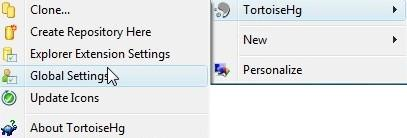
\includegraphics{cmenu-global-settings.jpg}
\caption{Open ``Global Settings'' from the desktop}\end{figure}

This opens the TortoiseHg settings dialog, editing your global (user)
configuration.  If you are using the command line, the global settings
dialog can be opened by \textbf{hgtk userconfig}.
\begin{figure}[htbp]
\centering

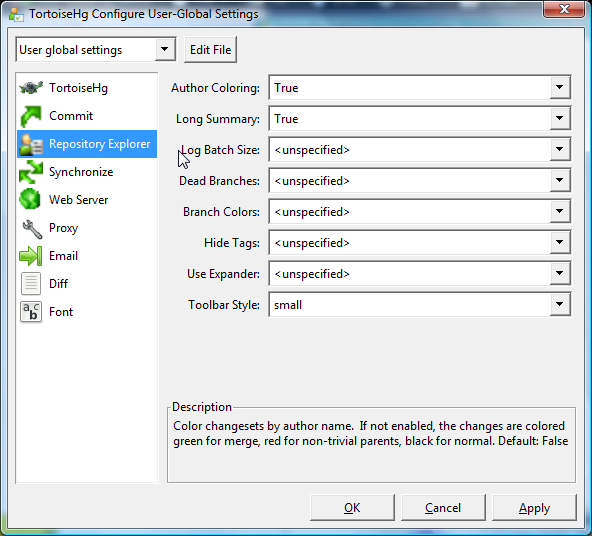
\includegraphics{settings.png}
\caption{TortoiseHg Settings Dialog}\end{figure}

First select the \textbf{Commit} page and enter a name in the
\textbf{Username} field.

\begin{notice}{note}{Note:}
If you neglect to configure a username TortoiseHg will ask you to
enter one when you try to \emph{commit}, which is the first time a
username is actually required.
\end{notice}

\begin{notice}{note}{Note:}
There are no hard fast rules on how to format your username, the
field is free form, but the following convention is commonly used:

\begin{Verbatim}[commandchars=@\[\]]
FullName @textless[]email@textgreater[]
\end{Verbatim}

for example

\begin{Verbatim}[commandchars=@\[\]]
Donald Duck @textless[]donaldduck@PYGZat[]example.net@textgreater[]
\end{Verbatim}

The email address is stripped when viewing history in the changelog
viewer, and the built-in web server obfuscates email addresses to
prevent SPAM.
\end{notice}

Next, select the \textbf{TortoiseHg} page and select the
\textbf{Three-way Merge Tool} entry.  In the drop down list you will
find all of the merge tools detected on your computer (kdiff3 is
provided by the Windows installer) and a number of internal merge
behaviors.  Select your preferred merge tool.

If you prefer for TortoiseHg to also use your selected merge tool for
visual diffs, you can leave the \textbf{Visual Diff Tool}
unspecified.  Otherwise, select your favorite visual diff tool from the
drop down list of detected visual diff tools.

If there are no options in either drop-down list, you must install a
diff/merge tool that is supported by our mergetools.rc or configure your
own tool.

\begin{notice}{note}{Note:}
If you installed TortoiseHg from source, you need to add our
contrib/mergetools.ini file to your HGRC path in some way.  One
approach is to \%include it from your \textasciitilde{}/.hgrc file.
\end{notice}

Feel free to configure other global settings while you have the dialog
open.  You will have the chance later to override these global settings
with repository local settings, if required.

Click the \textbf{Ok} button to save the changes you have made and
close the settings dialog.

\begin{notice}{note}{Note:}
Most TortoiseHg tools require a restart to pick up changes made in the
settings dialog.
\end{notice}


\section{Getting Acquainted}

Mercurial supports many different
\href{http://hgbook.red-bean.com/read/collaborating-with-other-people.html}{collaboration models}.
This chapter describes just one of those models: a single central repository.
The central repository model does not scale as well as other models, but
it is the most familiar to those coming from other revision tools and
thus is the most common approach people start with.

To get started, suppose you volunteer to create the central repository.
There are ways to \href{http://mercurial.selenic.com/wiki/RepositoryConversion}{convert}
non-Mercurial repositories into Mercurial repositories, but this example
assumes you are starting from scratch.


\section{Initialize the repository}

Create the initial repository on your local machine by using the
\textbf{Create Repository Here} shell menu option, or in a command
shell within the folder, type \textbf{hgtk init}.  You only need to do
this in once in the root folder of your project.
\begin{figure}[htbp]
\centering

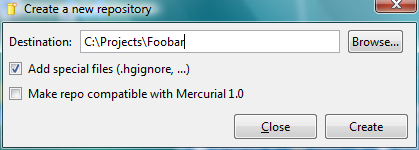
\includegraphics{init.png}
\caption{Repository Init Dialog}\end{figure}

We suggest you keep \textbf{Add special files (.hgignore, ...)}
checked, and do not check
\textbf{Make repo compatible with Mercurial 1.0}
unless you have a strong reason to do so.

After pressing \textbf{Create}, Mercurial creates a subdirectory in
your project folder named \code{.hg}. This is where Mercurial keeps all
its version data.  It is called the \emph{repository} or \emph{store}, while the
directory containing the source files is called the \emph{working directory}.
You never need to specify the \code{.hg} directory when running
commands, you only need to specify the working directory root.  It is
mentioned here just so you better understand how Mercurial works.

\begin{notice}{warning}{Warning:}
It is dangerous to manually edit the files in \code{.hg} directory,
repository corruption can occur.  \code{.hg/hgrc} is perhaps the
only exception to this rule.
\end{notice}


\section{Add files}

Now it's time to tell Mercurial which files must be tracked and which
files must be ignored. There are a lot of way to do this:
\begin{enumerate}
\item {} 
To add files, select them in explorer and then right click and select
\emph{TortoiseHg \(\rightarrow\) Add Files...} in the context menu. A
dialog will open for you to double check the selected files and
accept the add operation.

\item {} 
Or open the status tool (\emph{TortoiseHg \(\rightarrow\) View File Status}
or \textbf{hgtk status} from the command line). Check the files you
want to add and then press the \textbf{Add} button. From the
status tool you can launch the ignore filter tool from the context
menu of a unknown file (the menu option is named \textbf{ignore})

\item {} 
Or skip adding new files as a separate step and have the commit tool
add them implicitly.  The commit tool is very similar to the status
tool and allows you to do all of the same tasks. In this tool you
can add and commit an untracked file by just checking the file and
pressing \textbf{Commit}.

\item {} 
To ignore files, open the ignore filter dialog:
\emph{TortoiseHg \(\rightarrow\) Edit Ignore Filter} or from command
line \textbf{hgtk hgignore}. Choose a file from the list or
manually type in a \emph{Glob} or \emph{Regular expression} filter and then
press \textbf{Add}. Changes to the ignore filter take effect
immediately.

\end{enumerate}

\begin{notice}{note}{Note:}
The \code{.hgignore} file, contained in the working directory root,
is typically tracked (checked in).
\end{notice}

\begin{notice}{note}{Note:}
It is good practice to not have many \emph{unknown} files in your working
directory, as it makes it too easy to forget to add vital new files.
It is recommended that you keep your \code{.hgignore} file up to
date.
\end{notice}


\section{Commit}

Commit your local repository by right-clicking anywhere in the folder,
or on the folder itself, and then selecting \textbf{Hg Commit ...},
or from command line type \textbf{hgtk commit}.  Write a commit
message, select the files you wish to commit, then press
\textbf{Commit}. If, after the commit, you realize that something was
wrong with the message or the selected files, you can cancel the last
commit using the \textbf{Undo} button.  Your previous commit message
will be in the message history drop-down, so you do not have to type it
in again from scratch.

\begin{notice}{note}{Note:}
You lose the ability to easily undo the last commit when you close
the commit tool.
\end{notice}
\begin{figure}[htbp]
\centering

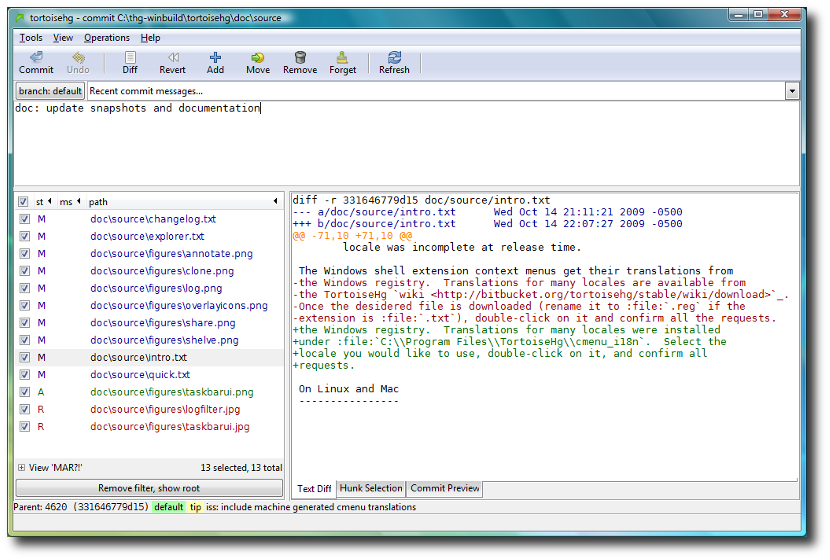
\includegraphics{commit.png}
\caption{Commit Tool}\end{figure}


\section{Share the repository}

Now you are ready to share your work. You do this by making a copy of
your repository in a public location that everyone in your group can
read. Mercurial calls this copy operation \emph{cloning your repository}. To
clone your repository to a shared drive, open the clone tool
\emph{TortoiseHg \(\rightarrow\) Clone a Repository}, or
\textbf{hgtk clone} from command line.  Then enter the destination
path.
\begin{figure}[htbp]
\centering

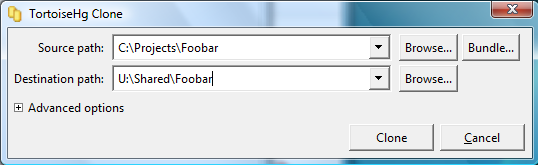
\includegraphics{share.png}
\caption{Clone Dialog}\end{figure}

When you create a clone for the purposes of generating a \emph{central
repository} there is no reason for that clone to have a working
directory. Checking
\textbf{do not update the new working directory} will prevent
Mercurial from checking out a working copy of the repository in the
central repository clone.  It will only have the \code{.hg} directory,
which stores the entire revision history of the project.

Other team members can clone from this clone with or without a checked
out working directory.


\section{Fetching from the group repository}

You want to start collaborating with your team.  They tell you something
like \emph{fetch the repository from x}.  What does that mean? It means that
you want to make a copy of the repository located at x on your local
machine.  Mercurial calls this cloning and TortiseHg has a dialog
for it. Right click in the directory where you want your copy and select
\emph{TortoiseHg \(\rightarrow\) Clone a Repository}, or
\textbf{hgtk clone} from command line.
\begin{figure}[htbp]
\centering

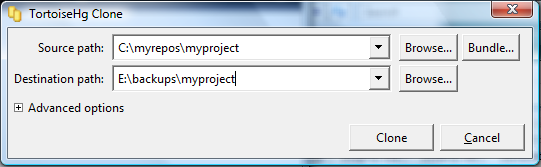
\includegraphics{clone.png}
\caption{Clone Dialog}\end{figure}

This time you do want to update the working directory because you want
to work on the project, uncheck
\textbf{do not update the new working directory} so Mercurial updates
the working directory with the \emph{tip} revision in your new clone.


\section{Working with your repository}

Suppose you've introduced some changes. It is easy to see that there are
a couple of directories with changes pending.  You can traverse the
directories to find specific changes and commit them from Explorer. A
quicker way is to use the commit tool:
\begin{figure}[htbp]
\centering


\includegraphics{overlayicons.png}
\caption{Overlay Icons on Vista}\end{figure}

The commit tool gives you a way to see differences or you can use your
visual difference tool (kdiff). Mercurial allows you to commit many
changes before you decide to synchronize (share changes) with the group
repository.

When you're ready to publish your changes, you
\begin{enumerate}
\item {} 
Commit your changes to your local repository (see above).

\item {} 
Pull changes from the group repository into your repository,
\emph{TortoiseHg \(\rightarrow\) Repository Browser} or
\textbf{hgtk log}, choose the path to the group repository
in the syncbar and then \textbf{Pull}.

\item {} 
If some changesets were pulled, merge those changes with your local
changes and then commit the merge into your local repository. From
the changelog viewer (\emph{TortoiseHg \(\rightarrow\) Repository Browser}
or \textbf{hgtk log}) open the context menu over the changeset
which you want to merge and select \textbf{merge with}.
Finally, in the merge dialog, press \textbf{Merge} and then
\textbf{Commit}.

\item {} 
Ensure your merged work still builds and passes your extensive test suite.

\item {} 
Push your changes to the group repository,
\emph{TortoiseHg \(\rightarrow\) Repository Browser} or \textbf{hgtk log},
choose the path to group repository and then \textbf{Push}.

\end{enumerate}

Which may sound complicated, but most of the time it is just pushing the
buttons in the commit and changelog tools.

\begin{notice}{note}{Note:}
Merges can be safely restarted if necessary.
\end{notice}

Mercurial makes collaboration easy, fast, and productive.
Learn more at Mercurial's \href{http://mercurial.selenic.com/wiki/}{wiki}.

\resetcurrentobjects
\hypertarget{--doc-daily}{}

\chapter{TortoiseHg in daily use}

\resetcurrentobjects
\hypertarget{--doc-common}{}

\section{Common Features}
\index{common.dialog (module)}
\hypertarget{module-common.dialog}{}
\declaremodule[common.dialog]{}{common.dialog}
\modulesynopsis{Common features to all the dialog}
These features are common to many TortoiseHg tools, so we document them
here just once.


\subsection{Keyboard Accelerators}

We define a few keyboard accelerators that all of the TortoiseHg tools support.
\begin{description}
\item[\code{Ctrl-Q}]
quit the application, including all open windows

\item[\code{Ctrl-W}]
close the current window (same as \code{Ctrl-Q} if only one window is open)

\item[\code{Ctrl-D}]
visual diff of currently selected file or changeset

\item[\code{Ctrl-Enter}]
activation

\item[\code{Ctrl-.} and \code{Ctrl-,}]
select next or previous file in a file list

\item[\code{Ctrl-{[}} and \code{Ctrl-{]}}]
page up or down a text pane

\item[\code{F5}, \code{Ctrl-R}]
refresh

\end{description}

On \href{http://bitbucket.org/tortoisehg/stable/wiki/MacOSX}{Mac OS X}, the
apple (command) key is used as the modifier instead of \code{Ctrl}.
However some keyboard accelerators are internal to GTK+ so you must use
the control key to access cut-paste functionality, for instance.


\subsection{Visual Diffs}
\begin{figure}[htbp]
\centering

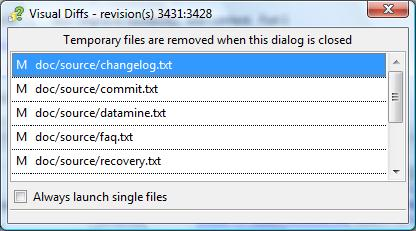
\includegraphics{visual-diff.jpg}
\caption{Visual Diff Window}\end{figure}

In TortoiseHg 1.0, the visual (external) diff infrastructure was
refactored.  The new system uses tool descriptions in
\code{mergetools.rc} to detect most common diff tools on your computer
(including KDiff3, which ships in our installer) and select the best
available tool.

If the user has selected a merge tool
(\emph{TortoiseHg \(\rightarrow\) Three-way Merge Tool}), that tool will
also be used to perform visual diffs, bypassing the tool selection
process.  However the user can still select a separate tool
(\emph{TortoiseHg \(\rightarrow\) Visual Diff Tool}) for visual diffs if
they chose.

The merge tool configuration file contains optimal command lines for
each tool, so no further configuration is required by the user.  They
only need to select the tools they wish use, or accept the defaults.

The visual diff system will use any existing extdiff configuration it
finds.  Since extdiff did not support three way diff arguments until
very recently and still does not support label arguments, you will
likely have a better experience by disabling or deleting any extdiff
configuration you may have.

The visual diff system will directly use the selected diff tool unless
the action you are attempting requires the use of the TortoiseHg visual
diff window.  The list of conditions includes:
\begin{enumerate}
\item {} 
The selection of files being compared require multiple tools

\item {} 
The selected tool forks detached background processes

\item {} 
The selected tool does not support the required directory diffs

\item {} 
The selected tool does not support three way comparisons

\item {} 
The file changes include renames or copies

\end{enumerate}

When the visual diff window is used, the temporary files are cleaned up
when the dialog is closed.  Thus it should be left open until you close
all of your diff tool instances.  When your diff tool is launched
directly, the temporary files are deleted when your tool exits.

If your diff tool is launched directly to compare a working copy file,
it will directly diff against the working file so you may modify it from
within the diff tool.  If you are comparing multiple files, the visual
diff system will make a snapshot of the working copy files and track
their initial sizes and timestamps.  When your diff tool exits, the
system compares the sizes and timestamps and copies modified files back
over the original working copies.  In this way, you can still modify
your working copy files from your visual diff tool even when performing
directory comparisons.

When the visual diff window is used to compare working copy files, it
always directly diffs against the working copy files since it always
operates on a single file at a time.

\begin{notice}{note}{Note:}
The \emph{TortoiseHg \(\rightarrow\) Skip Diff Window} configurable
has been removed because it is now redundant.
\end{notice}


\subsubsection{Adding Tools}

If you have a visual diff tool installed that is not supported by
TortoiseHg, you can create a tool configuration for it in your user
\code{Mercurial.ini} file.  See Mercurial's
\href{http://www.selenic.com/mercurial/hgrc.5.html\#merge-tools}{documentation}
on how to configure your tool for use in file merges.  When that is
complete, you can add the extra keys used by TortoiseHg for visual
diff:

\begin{Verbatim}[commandchars=@\[\]]
diffargs:  the arguments to use for two-way file comparisons
diff3args: the arguments to use for three-way file comparisons
dirdiff:   this tool supports two-way directory comparisons
dir3diff:  this tool supports three-way directory comparisons
\end{Verbatim}

When building command line arguments, you can use the following
variables:

\begin{Verbatim}[commandchars=@\[\]]
@$parent1:  the file or directory from the first parent revision
@$parent2:  the file or directory from the second parent revision
@$child:    the file or directory from the revision being compared
@$ancestor: the file or directory from the ancestor of a merge
@$parent:   a synonym for @$parent1

@$plabel1:  a symbolic name for the first parent revision
@$plabel2:  a symbolic name for the second parent revision
@$clabel:   a symbolic name for the revision being compared
@$alabel:   a symbolic name for the ancestor revision
\end{Verbatim}

Obviously, \$parent2 and \$ancestor are only meaningful when used in three
way diff arguments, for viewing merge changesets.  If your diff tool
cannot use the ancestor revision in any productive way, it is safe to
leave it out of the diff3args command line.

\begin{notice}{note}{Note:}
On Windows, the \emph{executable} parameter can use environment variables
using the syntax \$\{ProgramFiles\}
\end{notice}

If unconfigured, the default value of \textbf{diffargs} is `\$parent \$child'.
The default value of \textbf{diff3args} is ``'', indicating the visual diff
tool cannot perform three way comparisons.

If you create a new visual diff tool configuration, or improve upon an
existing configuration, please email it to our development mailing list
so it may be incorporated in a future release.


\subsubsection{Word Diffs}

The TortoiseHg Windows installers now include TortoiseSVN's scripts for
comparing (and sometimes merging) many binary document formats.  These
are configured in the site-wide \code{mergepatterns.rc} as handlers for
each binary format's common file extensions, so no user intervention is
required.

In order to support file extension based tool selection, TortoiseHg has
added support for a \textbf{{[}diff-patterns{]}} section equivalent to Mercurial's
\href{http://www.selenic.com/mercurial/hgrc.5.html\#merge-patterns}{merge-patterns}
section.


\subsection{Treeview searches}

Many TortoiseHg dialogs use treeviews to present lists of data to the
user. The file lists in the status, commit, shelve, and changelog tools
are treeviews. The changelog graph pane is a treeview. And even the
annotate pane in the datamine tool is a treeview.

Most of the TortoiseHg treeviews are configured for live searches.
Ensure that the treeview has focus (by clicking on a row), and begin
typing a search phrase. A small entry window will appear containing the
text you have typed, and the treeview will immediately jump to the first
row that matches the text you have entered thus far. As you enter more
characters, the search is refined. (Do not hit return to `complete' the
search, before using the keys mentioned below, or the entry window will
disappear, ending the search instead.)
\begin{itemize}
\item {} 
\code{Ctrl-F} opens the search window explicitly

\item {} 
\code{Ctrl-G} advances the search to the next match

\item {} 
\code{Shift-Ctrl-G} searches backwards

\item {} 
The mouse scroll wheel will advance forwards and backwards through
matching lines

\end{itemize}


\subsection{Hg command dialog}

Many TortoiseHg tools use the \emph{hgcmd} dialog to execute Mercurial
commands that could potentially be interactive.
\begin{figure}[htbp]
\centering

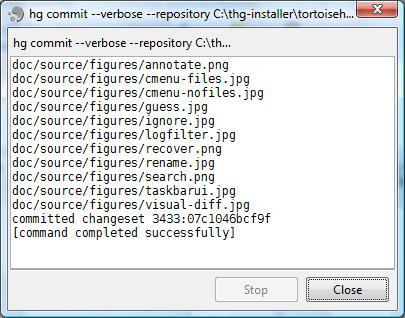
\includegraphics{hgcmd.jpg}
\caption{Interactive Mercurial Command Dialog}\end{figure}

\begin{notice}{note}{Note:}
Error messages are given a dark red color for contrast
\end{notice}

When the Mercurial command has completed, the dialog gives focus to its
\textbf{Close} button.  So pressing \code{Enter} is all that is
required to close the window.

\resetcurrentobjects
\hypertarget{--doc-explorer}{}

\section{Windows Explorer Integration}
\index{explorer (module)}
\hypertarget{module-explorer}{}
\declaremodule[explorer]{}{explorer}
\modulesynopsis{Windows explorer integration}

\subsection{Overlay Icons}

TortoiseHg provides visual representation of the file status via overlay
icons in the MS-Explorer windows. This is similar to those that found on
other Tortoise client, such as TortoiseCVS and TortoiseSVN.

TortoiseHg shares the overlay icons with TortoiseSVN (version 1.5.x or
later) and the other ``Tortoise'' projects via the use of TortoiseOverlays
(another project created by TortoiseSVN team).
\begin{figure}[htbp]
\centering


\includegraphics{overlayicons.png}
\caption{Overlay icons in Icons view (XP)}\end{figure}

The context menu has an \textbf{Update Icons} option which forces
TortoiseHg to refresh the icons in the currently browsed repository or
directory of repositories. The taskbar icon will turn green and the
directory icons will turn into question marks while this refresh is in
progress.

The overlay handler and context menus are configurable.  From any folder
background (even the desktop), right click and select
\emph{TortoiseHg \(\rightarrow\) Explorer Extension Settings}. In the settings
dialog you can promote individual menu options to the top menu.
\begin{figure}[htbp]
\centering

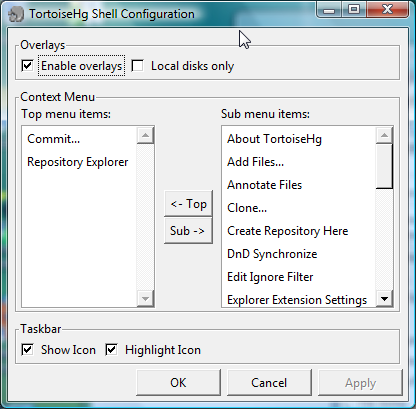
\includegraphics{taskbarui.png}
\caption{Shell Configuration Dialog}\end{figure}

One can selectively disable overlay icons in a specific repository by
editing the \code{.hg\textbackslash{}thgstatus} file inside the repository and
replacing it's contents with a single line containing:

\begin{Verbatim}[commandchars=@\[\]]
@PYGZat[]@PYGZat[]noicons
\end{Verbatim}


\subsection{Context Menus}

TortoiseHg commands may be accessed via the context menu of Explorer
windows and other applications which use the standard File/Open dialogs.
Here is the context menu for a revisioned folder:
\begin{figure}[htbp]
\centering

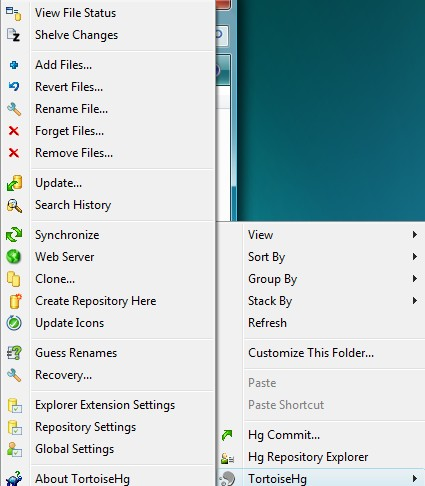
\includegraphics{cmenu-nofiles.jpg}
\caption{Context menu for a folder under Mercurial revision control}\end{figure}

And here is the context menu for selected files or folders:
\begin{figure}[htbp]
\centering

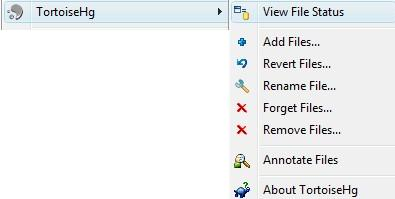
\includegraphics{cmenu-files.jpg}
\caption{Context menu for file or folder selection}\end{figure}

TortoiseHg provides dialogs for the most regularly used Mercurial
commands.  Less frequently used and newly added Mercurial commands
may be accessed from the CLI (command line interface) through
\code{cmd.exe} on Windows.


\subsection{Nautilus}

TortoiseHg also provides shell integration with the GNOME desktop via a
nautilus-python plugin.  If you have installed TortoiseHg from a
distribution package, the odds are that this extension is already
configured.  If not, please consult our Wiki for instructions on how to
enable this feature.

While the nautilus extension does not have it's own GUI for managing the
overlays and context menus, it does support command promotion into the
top menu.  It requires you to edit your \code{\textasciitilde{}/.hgrc} file and add
lines like these:

\begin{Verbatim}[commandchars=@\[\]]
@PYGZlb[]tortoisehg@PYGZrb[]
promoteditems @PYGbe[=] commit, log, synch
\end{Verbatim}
\begin{figure}[htbp]
\centering

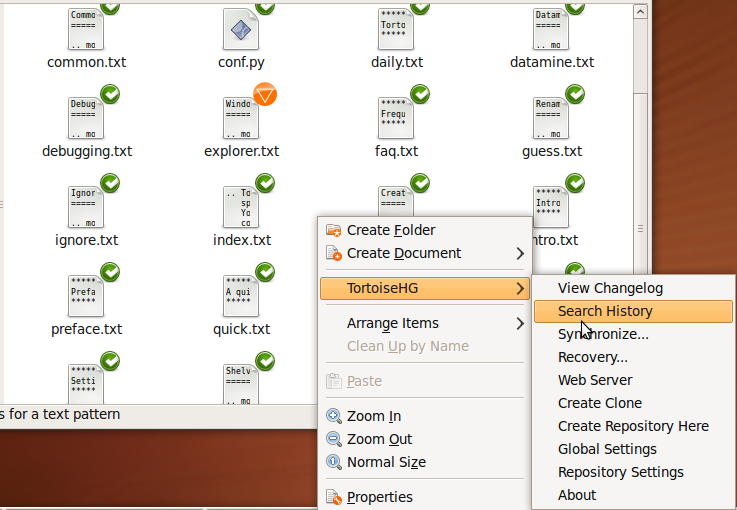
\includegraphics{nautilus.png}
\caption{GNOME/Nautilus screenshot}\end{figure}

\resetcurrentobjects
\hypertarget{--doc-init}{}

\section{Create a new repository}
\index{init.dialog (module)}
\hypertarget{module-init.dialog}{}
\declaremodule[init.dialog]{}{init.dialog}
\modulesynopsis{Dialog used to create a repository}
To create a new repository into an existing directory (project) you
have to run the init dialog. From the explorer context menu select
\emph{TortoiseHg... \(\rightarrow\) Create Repository Here} over the directory, or, within
the folder, type \textbf{hgtk init}.
\begin{figure}[htbp]
\centering

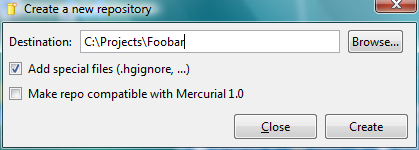
\includegraphics{init.png}
\caption{Repository Init Dialog}\end{figure}
\begin{description}
\item[\textbf{Destination}]
Is the directory where the repository will be created. It is
always filled with the current directory, so if you launch the
dialog from the right directory there is no reason to change it.

\item[\textbf{Add special files (.hgignore, ...)}]
If selected TortoiseHg creates an empty \code{.hgignore} file
in the working directory.

\item[\textbf{Make repo compatible with Mercurial 1.0}]
If selected TortoiseHg creates an older format Mercurial repository.
Do not check unless you have a strong reason to do, and you know
what you are doing.

\end{description}

Creating a new repository means create a subdirectory called \code{.hg}.
In this subdirectory Mercurial keeps all its versioning information.

\begin{notice}{warning}{Warning:}
It is dangerous to manually edit the files in \code{.hg} directory,
repository corruption can occur.  \code{.hg/hgrc} is perhaps the
only exception to this rule.
\end{notice}


\subsection{From command line}

The init tool can be started from command line

\begin{Verbatim}[commandchars=@\[\]]
hgtk init
\end{Verbatim}

The syntax is

\begin{Verbatim}[commandchars=@\[\]]
hgtk init @PYGZlb[]DEST@PYGZrb[]
\end{Verbatim}

where {[}DEST{]} is the path to destination folder.

\resetcurrentobjects
\hypertarget{--doc-clone}{}

\section{Clone a repository}
\index{clone.dialog (module)}
\hypertarget{module-clone.dialog}{}
\declaremodule[clone.dialog]{}{clone.dialog}
\modulesynopsis{Dialog used to clone a repository}
To clone a repository you have to run the clone dialog.
From the explorer context menu select \emph{TortoiseHg... \(\rightarrow\) Clone a repository}
or type \textbf{hgtk clone}.
\begin{figure}[htbp]
\centering

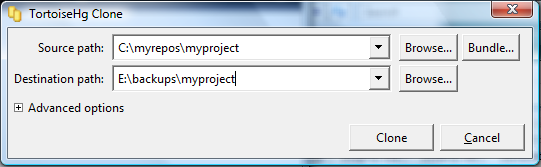
\includegraphics{clone.png}
\caption{Clone Dialog}\end{figure}
\begin{description}
\item[\textbf{Source Path}]
It is the path (or URL) of the repository that will be cloned. Use
the \textbf{Browse...} to choose a local folder.

\item[\textbf{Destination Path}]
It is the path of destination directory, a folder with the same name
of source repository will be created within this directory.

\end{description}

Under the \textbf{Advanced options} expander you will find:
\begin{description}
\item[\textbf{Clone To Revision}]
You can limit the clone up to this revision. Even the tags created
after this revision will not be imported.

\item[\textbf{do not update the new working directory}]
If checked, after the clone the working directory will be empty. It
is useful when you have to clone a repository with the purpose of
central repository, or backup, where you have only, in the future,
to \emph{push} and \emph{pull}.

\item[\textbf{use pull protocol to copy metadata}]
When the source and destination are on the same filesystem,
Mercurial tries to use hardlinks. Some filesystems, such as AFS
implement hardlink incorrectly, but do not report errors. Use this
option to avoid hardlinks.

\item[\textbf{use uncompressed transfer}]
To use uncompressed transfer (fast over LAN).

\item[\textbf{use proxy server}]
To use the proxy server configured in \emph{TortoiseHg... \(\rightarrow\) Global Settings \(\rightarrow\) Proxy}.
This is enabled only if a proxy is configured.

\item[\textbf{Remote Cmd}]
Specify a Mercurial command to run  on the remote side.

\end{description}


\subsection{From command line}

The clone tool can be started from command line

\begin{Verbatim}[commandchars=@\[\]]
hgtk clone
\end{Verbatim}

The syntax is

\begin{Verbatim}[commandchars=@\[\]]
hgtk clone @PYGZlb[]SOURCE@PYGZrb[] @PYGZlb[]DEST@PYGZrb[]
\end{Verbatim}

where {[}SOURCE{]} and {[}DEST{]} are, the paths of source repository and destination folder.

\resetcurrentobjects
\hypertarget{--doc-commit}{}

\section{Commit}
\index{commit.dialog (module)}
\hypertarget{module-commit.dialog}{}
\declaremodule[commit.dialog]{}{commit.dialog}
\modulesynopsis{Dialog used to perform commit}
\begin{notice}{warning}{Warning:}
The win32text extension can cause trouble with hunk selection.  This
has been resolved in Mercurial 1.3 and TortoiseHg 0.8, but requires
proper configuration. See
\href{http://bitbucket.org/tortoisehg/stable/issue/82/}{issue \#82}.
\end{notice}

The commit tool is one of the two main applications of TortoiseHg.
Together with the Repository Explorer (aka, the changelog tool) these
two tools can perform or access nearly every function that TortoiseHg
supports.

Not only can the commit tool commit your changes, but it can also
examine the state of your working directory and perform most routine
maintenance tasks (add new files, record renames, manage the ignore
filter, etc).
\begin{figure}[htbp]
\centering

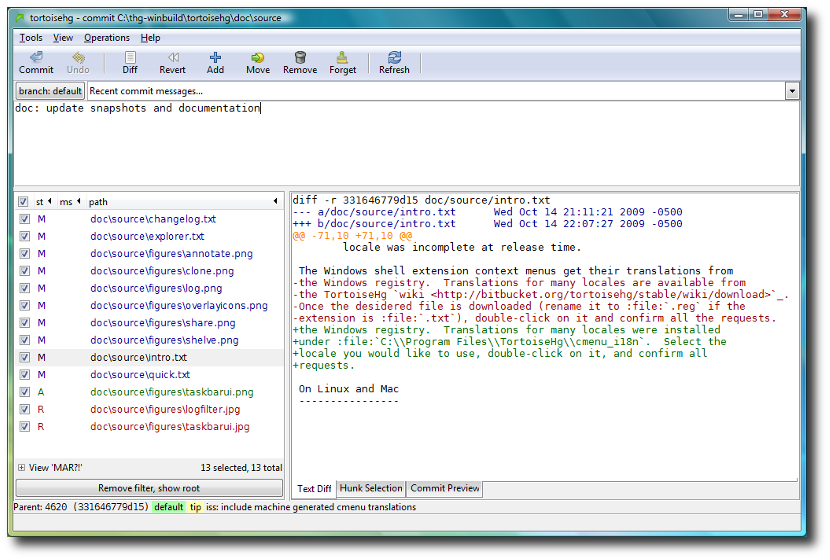
\includegraphics{commit.png}
\caption{Commit dialog}\end{figure}


\subsection{Features}

At the top of the commit tool is a menu bar, newly introduced in version 0.9.
\begin{quote}
\begin{description}
\item[\textbf{Tools}]
Launch common TortoiseHg tools in separate processes

\item[\textbf{View}]
Toggle the display of optional features, or refresh the working
directory contents.

\item[\textbf{Operations}]
These menu items correspond to the toolbar buttons.

\item[\textbf{Help}]
Open a web browser to this web page, or launch TortoiseHg About
dialog.

\end{description}
\end{quote}

Enumerating the toolbar buttons:
\begin{quote}
\begin{description}
\item[\textbf{Commit}]
Commit selected diffs in checked files.

\item[\textbf{Undo}]
Undo (rollback) last immediate commit. Your commit message will be
available in the message history, so you can easily repeat the
commit if necessary.

\item[\textbf{Diff}]
Visual diff checked files.

\item[\textbf{Revert}]
Revert checked files to last revisioned state.  If merging, it
allows you to select the revert parent.

\item[\textbf{Add}]
Add checked files that were in unknown `?' or ignored `I' state.

\item[\textbf{Move}]
Move checked files to specified target directory in versioned
manner.

\item[\textbf{Remove}]
Delete checked unversioned files and/or remove (mark as deleted) any
versioned files.

\item[\textbf{Forget}]
Forget checked versioned files.

\item[\textbf{Refresh}]
Reload the state of the working directory. It tries to retain
check and selection state across refresh.

\item[\textbf{Patch Queue}]
If the MQ extension is enabled, this toggle button for the patch
queue pane will be visible.

\end{description}
\end{quote}

Below the toolbar are useful widgets:
\begin{quote}
\begin{description}
\item[\textbf{Branch dialog}]
Shows the current branch name of the working directory. Normally
this is informational only, but pressing this button opens up a
branch maintenance dialog.  Do not use this feature unless you
understand Mercurial's
\href{http://mercurial.selenic.com/wiki/NamedBranches}{named branches}.

\item[\textbf{Recent Commit Messages}]
A drop-down list of the 10 most recent commit messages. The
the drop-down list is filled the first time it is opened.

\item[\textbf{QNew}]
If you have enabled the MQ extension, there will also be a text
entry for a new patch name.  Entering a patch name switches the
commit tool into `QNew' mode.

\end{description}
\end{quote}

The file list has four columns:
\begin{enumerate}
\item {} 
A checkbox that indicates whether the file is selected for an
operation.  The toolbar buttons only operate on checked files.
``Partially'' selected files have a special check state.  This
column header is checkable, it will toggle the file selection
states.

\item {} 
The \textbf{st} column holds the status of the file, defined
by Mercurial's status command, one of `MARD?IC'.  A status of `S'
indicates a dirty subrepository that needs to be committed.

\item {} 
The \textbf{ms} column holds the merge state of the file,
defined by Mercurial's resolve command, one of ` RU'.  See the
merge section below.

\item {} 
The canonical path of the file relative to the repository root

\end{enumerate}

\begin{notice}{note}{Note:}
If the commit tool was started with a file pattern or selection, a
button will appear at the bottom of the file list that can clear the
file pattern and give you an unfiltered view of the entire working
directory.
\end{notice}

Below the file list, inside an expander, are checkboxes that toggle the
display of the various classes of files \{modified, added, removed,
deleted, unknown, clean, ignored\}.  These check boxes will be disabled
if the commit tool was started with a file pattern or selection.

\emph{Removed} means a revisioned file has been marked as removed. \emph{Deleted}
means a revisioned file is missing but Mercurial has not been told to
quit tracking that file. For instance, if you rename a revisioned file
in the explorer, the original filename will show up as deleted and the
new filename will show up as unknown. By right-clicking on the new
filename you can bring up the rename guessing dialog which can discover
the rename by comparing file contents and mark the old file as removed
and the new file as added while recording the whole operation as a
rename.

\emph{Unknown} files are not tracked by Mercurial, but they also do not match
any ignore filters you have configured.  Unknown files are shown by
default because they are usually files that need to be added to revision
control.  It is recommended that you keep your ignore filters up to date
to ensure that is the case.  The context menu of unknown files has an
option open the ignore pattern tool.

\emph{Clean} files are tracked files that have not been modified, while
\emph{Ignored} files are untracked files that match a configured ignore
pattern.  Neither of those file types are shown by default, unless a the
user includes such a file in a selection (explorer) or provides the file
name on the command line.
\begin{figure}[htbp]
\centering

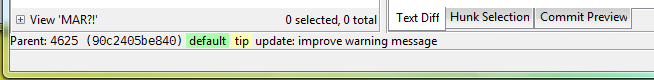
\includegraphics{parentbar.png}
\caption{Parent bar in commit dialog}\end{figure}

Below both the file list and diff pane is a narrow
\textbf{Parents Bar}.  This bar shows you the current working
directory parent(s), and gives you some warnings if a commit would
introduce a new head.  The parents bar can be hidden by an option in the
\textbf{View} menu.

To the right of the file list is the diff pane.  The diff pane is newly
tabbed in the 0.9 release.
\begin{quote}
\begin{description}
\item[\textbf{Text Diff}]
Shows the textual diffs in the currently selected file.

\item[\textbf{Hunk Selection}]
In releases 0.7 through 0.8, this tab was the only content shown
to the user.  The diffs in this tab can be toggled per ``hunk'',
allowing the user to cherry pick changes to be included in the
commit.  As in 0.8, this tab only shows diff hunks for the
currently selected file.  This tab cannot show binary diffs or
renames.  That data can only be seen in the Text Diff tab.

\item[\textbf{Commit Preview}]
This tab previews all of the selected hunks in every checked
file, essentially a preview of what will be committed when you
press the commit button.

\item[\textbf{Patch Contents}]
Only visible when the commit tool is in QRefresh mode.  It
displays the current contents of the patch being refreshed.

\end{description}
\end{quote}
\begin{figure}[htbp]
\centering

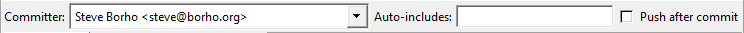
\includegraphics{advancedbar.png}
\caption{Advanced bar in commit dialog}\end{figure}

If the \textbf{Advanced Bar} is enabled in the \textbf{View} menu,
a bar is inserted between the toolbar and the message history bar.  The
advanced bar contains:
\begin{quote}
\begin{description}
\item[\textbf{Committer}]
The username to use for this commit.  This value is usually read
from your Mercurial.ini file, but it can be specified on the
hgtk command line or read from a patch file.  Lastly, the user
could manually specify a different username here.

\item[\textbf{Auto-includes}]
A text entry that allows the user to modify the comma separated
list of files that are always included in the commit list,
regardless of whether they have been checked.  This is intended
for use in repositories that have pre-commit hooks that modify
certain files (say a changelog).

\item[\textbf{Push after commit}]
A toggle button that determines whether TortoiseHg will attempt
to push outgoing changes to your default push target after each
successful commit.

\end{description}
\end{quote}


\subsection{Change Selection}

So what does the phrase `commit the selected diffs in checked files'
mean?  Simple, the TortoiseHg commit tool supports change selection
intrinsically in the diff browser. This means that all of the changes
you make to versioned files can be individually selected to be included
in the commit or left out of the commit (but left in the working
directory).  Fans of darcs or Mercurial's record extension will
recognize this feature immediately.


\subsubsection{When is this necessary?}

When you have more than a single coherent change in your source code and
you would like to commit your changes piecemeal.  This can often be
accomplished by filtering the list of files in each commit, but there
will be times when your changes intermingle in the same set of files and
that is when this change selection feature becomes indispensable.


\subsubsection{How does it work?}

By double-clicking on individual change hunks in the
\textbf{Hunk Selection} tab of the diff panel.  \emph{Technically, any
action which activates a change hunk row will toggle it's selection
status. The spacebar will also work.} When a hunk is unselected, the
syntax highlighting of the diff is disabled and the background is turned
gray.  At the same time, the file's diff header is updated to show the
current selection state, the selected hunk count and changed lines will
be updated. Toggle the hunk a second time to reselect it for inclusion
in your commit.

When a file is partially selected for commit, it's icon is changed from
a checkbox to a radio button. At a glance at the file list, you should
be able to find which files are entirely included in the commit,
partially included, or entirely excluded.


\subsubsection{What happens at commit time?}

The short answer is that the selected hunks in checked files are
committed to the repository and the unselected changes are left in your
working directory for the next commit.

The long answer is a little more complicated.  What happens behind the
scenes is that the files which are partially selected are backed up in a
safe location, reverted to their last revisioned state, have their
selected change hunks applied back to them, committed, and then finally
recovered from backup (thus placing the rejected change hunks back into
the working copy).  Files which are not partially selected avoid the
entire \emph{backup, revert, patch, commit, recover} round trip and instead
are committed in place.

This longer answer is only interesting when something goes wrong, which
on Windows unfortunately has a probability greater than 0. If some
program (virus checker, compiler) locks your file in the middle of this
process you may see an error about a failed patch.  These errors are
recoverable.  Delete any new \code{.rej} files left in your repository
and retry the commit.


\subsection{Keyboard navigation}
\begin{description}
\item[\code{Ctrl-Enter}]
Trigger the commit

\item[\code{Ctrl-C}]
When pressed in the diff panel, ctrl-c will copy the currently
highlighted (repeat highlighted, not selected) diff hunks to the
clipboard. These can be pasted into a text buffer to generate any
arbitrary patch based from the changes in your working directory.

\item[\code{Alt-Q}]
Reflow the paragraph currently under the cursor.  You must configure
a message format policy for this key combination to work.

\end{description}

The code which copies the hunks to the clipboard is intelligent about
diff headers.  The clipboard contents will always be a valid patch.


\subsection{File Context Menus}

When right clicking on files in the file list, you will get a context
menu of commands that are applicable to the selected files.

For unknown \textbf{?} files, the context menu will allow you to detect
renames (if you think the unknown file is a copy or rename of a
revisioned file) or to configure the repository's ignore filter (if the
unknown file should never be revisioned and you want Mercurial to ignore
it).


\subsection{Merging}

The commit tool has a special mode when it is opened in a repository
that is in a merged state (technically, this means the current working
directory has two parent revisions). The file list has no checkboxes and
the hunk selection tabs are hidden. The commit `manifest' is essentially
immutable, since you must commit the entire working directory after a
merge.

The merge state \emph{ms} column is especially useful in this mode.  Files
that are marked with \emph{R} are files where Mercurial and/or the user have
successfully merged (resolved) changes from both parents. Files that
are marked with \emph{U} have unresolved changes. You can use the \emph{Restart
Merge} context menu option to restart the merge for those files, or you
can use the \emph{edit} context menu option to resolve the conflict by hand.
The \emph{Restart Merge} menu option allows you to select the merge tool to
use to perform the merge, or even to pick one version or the other
unconditionally (internal:local, internal:other).  After the conflicts
have been manually resolved, you must use the \emph{mark resolved} context
menu option to change the file's merge state to \emph{R}.

Mercurial will not allow you to commit a merge if any files have
unresolved \emph{U} merge states.

For your reference, \emph{local} is the revision you had checked out when you
started the merge and \emph{other} is the revision you merged with.

To undo a failed merge attempt, you must tell Mercurial to remove the
second parent from your working directory.  This usually means
performing a clean update of the first parent.  The merge tool has an
\textbf{Undo} button which does exactly that.  The recovery tool also
has a \textbf{Clean} button that does the same thing.

Once you have your working directory back at one parent revision, you
may restart the merge process.


\subsection{Commit Message Pane}

The commit message pane has these special context menu options:
\begin{quote}
\begin{description}
\item[\textbf{Paste Filenames}:]
Paste checked filenames into the commit message at the cursor.

\item[\textbf{Apply Format}:]
Apply configured message wrap policy to current message.

\item[\textbf{Configure Format}:]
Opens the settings dialog to the \textbf{Commit} tab.

\end{description}
\end{quote}

If your project has guidelines for the format of commit messages, you
can configure them in the settings tool.  The commit tool will enforce
your policy at commit time, and you can ask the tool to apply the format
to the current message.  The \textbf{Commit} tab of the settings tool
has these two configurables for commit message policy:
\begin{quote}
\begin{description}
\item[\textbf{Summary Line Length}:]
Maximum length of the commit message summary line.  If set,
TortoiseHg will issue a warning if the summary line is too long
or not separated by a blank line. Default: 0 (unenforced)

\item[\textbf{Message Line Length}:]
Word wrap length of the commit message.  If set, the popup menu
can be used to format the message and a warning will be issued
if any lines are too long at commit.  Default: 0 (unenforced)

\end{description}
\end{quote}


\subsection{Subrepositories}

A \href{http://mercurial.selenic.com/wiki/subrepos}{subrepository}
is a feature introduced in Mercurial 1.3.  It allows one Mercurial
repository to store references to external Mercurial (or potentially
other VCS) repositories, and to include the state of those external
repositories in the main repository's history.

TortoiseHg 1.0 introduced rudimentary support for subrepositories, and
only in the commit / status tool.  When Mercurial considers a subrepo as
dirty, it will appear in the commit tool as a special entry in the file
list with a status of \emph{S}.  If a subrepo is included in the file list of
a commit, the subrepo is committed along with the other changes,
updating the .hgsubstate file in the main repository root.

Prior to TortoiseHg 1.0, dirty subrepos were not shown in the commit
tool and .hgsubstate was not updated during commits.


\subsection{MQ patches}

Many advanced Mercurial users use the MQ extension to manage a patch
queue.  The commit tool will recognize when a patch is applied and enter
\emph{patch refresh} mode. The title bar will say ``refreshing patch
\emph{patchname}'' and the patch comment will appear in the commit message
pane.

A new `Patch Contents' tab will appear in the diff pane with the full
contents of the top patch.  The Text Diff and Hunk Selection tabs will
show the combined diff of the patch and working directory changes so
that you can move changes into or out of the patch during the qrefresh.

This is essentially what the qdiff command would show you.  There is, in
fact, no way to get just the working copy diffs beyond running
\textbf{hg diff} on the command line or typing a name into the QNew
entry which toggles the dialog into QNew mode (more below).

The \textbf{Commit} button, which has been renamed \textbf{QRefresh}
in this context, will refresh the top patch with the changes you
have selected, including the patch description. This may be a bit
confusing at first because the changes you leave out of the patch are
still going to be in the working directory after the refresh, so unless
you look at the patch contents it will not seem as if anything changed.


\subsection{QNew Mode}

The commit tool can be used to create a new patch for your patch queue.
If you have the MQ extension enabled, a text entry will be inserted
between the branch maintenance button and the message history drop-down
box.  If you enter a filename in this entry the commit tool will switch
out of \emph{commit} or \emph{qrefresh} mode into \emph{qnew} mode.  In \emph{qnew} mode,
the commit tool shows only working directory modifications (the changes
that would typically get added to a new patch by \textbf{hg qnew -f}).
The \textbf{Commit} button will change into a \textbf{QNew} button
as well, to make the mode switch more obvious.

When the \textbf{QNew} button is pressed, the selected change hunks
are written into a new patch (given the filename you specified), and the
dialog is refreshed.  After this refresh, the commit tool will obviously
switch to \emph{qrefresh} mode since there will now be at least one applied
patch.

You may give the new patch a commit message at the initial \emph{qnew} event,
or you can do it afterwords while in \emph{qrefresh} mode.


\subsection{Configurables}
\begin{description}
\item[\emph{Commit \(\rightarrow\) Username}]
Sets username associated with your commits (see \hyperlink{--doc-quick}{\emph{A Quick Start Guide to TortoiseHg}})

\item[\emph{Commit \(\rightarrow\) Summary Line Length}]
Configures a `policy' limit for summary lines

\item[\emph{Commit \(\rightarrow\) Message Line Length}]
Configures a `policy' limit for message lines

\end{description}

And three other features for \emph{advanced} users.
\begin{description}
\item[\emph{Commit \(\rightarrow\) Push After Commit}:]
When set to True, the commit tool will check the \emph{push after
commit} toggle button on startup.

\item[\emph{Commit \(\rightarrow\) Auto Commit List}:]
Comma separated list of files that are automatically included in
every commit.  Intended for use only as a repository setting.

\item[\emph{Commit \(\rightarrow\) Auto Exclude List}:]
Comma separated list of files that are automatically unchecked
when the status, commit, and shelve tools are opened.

\item[\emph{TortoiseHg \(\rightarrow\) Bottom Diffs}]
Toggles diff pane from left to below file list

\item[\emph{TortoiseHg \(\rightarrow\) Max Diff Size}]
Configures the diff size limit

\end{description}

External tool configuration has been removed in 0.9


\subsection{From command line}

The commit tool can be started from command line:

\begin{Verbatim}[commandchars=@\[\]]
hgtk commit @PYGZlb[]OPTIONS@PYGZrb[] @PYGZlb[]FILE@PYGZrb[]...

aliases: ci

commit tool

options:

 -u --user  record user as committer
 -d --date  record datecode as commit date

use "hgtk -v help commit" to show global options
\end{Verbatim}

For a quick help on the format of date type:

\begin{Verbatim}[commandchars=@\[\]]
hg help dates
\end{Verbatim}

\resetcurrentobjects
\hypertarget{--doc-shelve}{}

\section{Shelve}
\index{shelve.dialog (module)}
\hypertarget{module-shelve.dialog}{}
\declaremodule[shelve.dialog]{}{shelve.dialog}
\modulesynopsis{Dialog used to perform shelve/unshelve operations}
\begin{notice}{warning}{Warning:}
The win32text extension can cause trouble with hunk selection.  This
has been resolved in Mercurial 1.3 and TortoiseHg 0.8, but requires
proper configuration. See
\href{http://bitbucket.org/tortoisehg/stable/issue/82/}{issue \#82}.
\end{notice}

The purpose of this dialog is to allow the user to \emph{shelve} selected changes
from the working directory, store them in a special patch file within the
repository, and then \emph{unshelve} them back at a later time.
\begin{figure}[htbp]
\centering

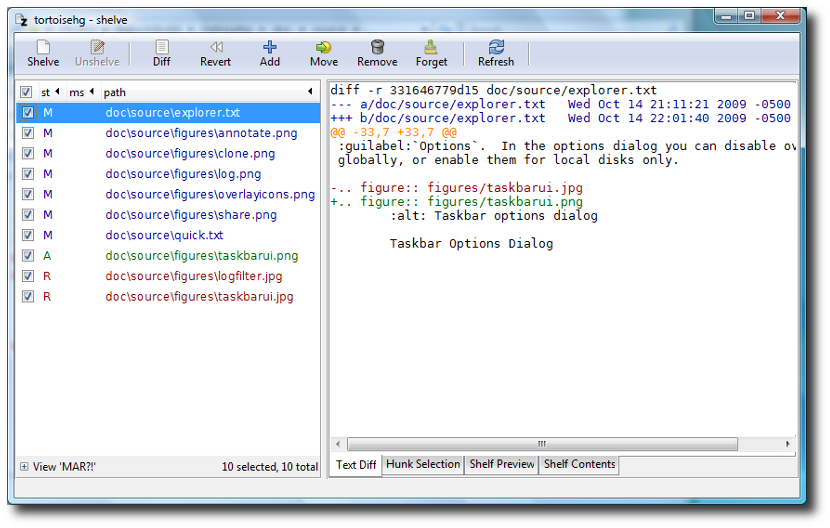
\includegraphics{shelve.png}
\caption{Shelve dialog}\end{figure}

Walking across the toolbar buttons:
\begin{quote}
\begin{description}
\item[\textbf{Shelve}]
Shelve selected diffs in checked files.

\item[\textbf{Unshelve}]
Replace the shelved changes back into the working directory.

\item[\textbf{Diff}]
Visual diff checked files

\item[\textbf{Revert}]
Revert checked files to last revisioned state.  If merging, it
allows you to select the revert parent.

\item[\textbf{Add}]
Add checked files that were in unknown `?' or ignored `I' state.

\item[\textbf{Move}]
Move checked files to specified target directory in versioned
manner.

\item[\textbf{Remove}]
Delete checked unversioned files and/or remove (mark as deleted) any
versioned files.

\item[\textbf{Forget}]
Forget checked versioned files

\item[\textbf{Refresh}]
Reload the state of the working directory. It tries to retain
check and selection state across refresh.

\end{description}
\end{quote}

The file list has four columns:
\begin{enumerate}
\item {} 
A checkbox that indicates whether the file is selected for an
operation.  The toolbar buttons only operate on checked files.
``Partially'' selected files have a special check state.  This
column header is checkable, it will toggle the file selection
states.

\item {} 
The \textbf{st} column holds the status of the file, defined
by Mercurial's status command, one of `MARD?IC'.

\item {} 
The \textbf{ms} column holds the merge state of the file,
defined by Mercurial's resolve command, one of ` RU'.

\item {} 
The canonical path of the file (relative to the repository root)

\end{enumerate}

Below the file list are checkboxes that toggle the display of the
various classes of files \{modified, added, removed, deleted, unknown,
clean, ignored\}.  These check boxes will be disabled if the commit tool
was given a specific set of files and/or directories.


\subsection{Tabs}
\begin{description}
\item[The shelve tool diff pane has four tabs]\begin{enumerate}
\item {} 
Text Diff - shows diff of currently selected file

\item {} 
Hunk Selection - allows diff hunks of current file to be skipped

\item {} 
Shelf Preview - displays all selected changes. This previews the
changes that will be removed from the working directory and
stored in the shelf.

\item {} 
Shelf Contents - the current contents of the shelf.

\end{enumerate}

\end{description}


\subsection{Shelving Changes}

Just like the commit tool, this dialog uses TortoiseHg's integrated hunk
selection code to allow the user to select the files and change hunks to
move to the shelf.  When you press the shelve button, the selected
changes are removed from the working directory and placed in a patch
file. If the shelf already had changes in it, you will be asked whether
to replace those changes or to merge these new changes into it.  When
the shelf has changes, the unshelve button will be active.


\subsection{Unshelving Changes}

When the unshelve button is pressed, the shelved changes are reapplied
to the working directory.

\begin{notice}{note}{Note:}
The unshelved changes will appear as working directory modifications
when the shelve tool refreshes it's view of the repository.
\end{notice}


\subsubsection{How is this different from record/commit?}

Shelved changes are physically removed from the working directory until
you unshelve them.  This means you can build your project and run tests
on it while the shelved changes are gone.  This is safer than selecting
changes at build time since you can test whether the change being
committed is valid.

Shelving changes is also useful for removing partially completed work to
make sure it doesn't interfere with the debugging of other changes you
are making.

Caveat: the shelved changes are stored in a patch that is based on the
current working directory contents. There's no guarantee that the patch
can be cleanly reapplied later if the shelved changes conflict with
changes made to your code after the shelving.


\subsubsection{How is this different from MQ?}

The shelf can be considered a single unnamed MQ patch that is never
converted into a changeset.

The shelve tool can be useful when maintaining a patch queue.
The shelf can take changes from one patch and re-apply them to another
patch (or an entirely new patch).
\begin{description}
\item[For example:]\begin{enumerate}
\item {} 
Push to a patch you would like to split up

\item {} 
Open the shelve tool, the top patch changes will be selectable

\item {} 
Unselect change hunks you want to leave in the patch, then press
\textbf{Shelve}

\item {} 
Refresh top patch using \textbf{hg qrefresh}, or use commit tool

\item {} 
Push or pop to the patch you want to apply shelved patches

\item {} 
Open the shelve tool and press \textbf{Unshelve}

\item {} 
Refresh top patch (repeat step 4)

\end{enumerate}

\end{description}

You cannot shelve added, removed, or renamed files, but MQ can handle
this just fine.


\subsubsection{How is this different from attic?}

The attic extension is a super-set of the shelve feature. In particular,
attic allows you to have several named \emph{shelves} which can be saved and
restored independently.


\subsection{Keyboard navigation}
\begin{description}
\item[\textbf{Ctrl-C}]
in the diff panel will copy the currently highlighted (not selected,
but highlighted) diff hunks to the clipboard. These can be pasted
into a text buffer to generate any arbitrary patch based from the
changes in your working directory.

\end{description}

The code which copies the hunks to the clipboard is intelligent about
diff headers.  The clipboard contents will always be a valid patch.


\subsection{Configurables}
\begin{itemize}
\item {} 
\emph{TortoiseHg \(\rightarrow\) Bottom Diffs}

\item {} 
\emph{TortoiseHg \(\rightarrow\) Tab Width}

\item {} 
\emph{TortoiseHg \(\rightarrow\) Max Diff Size}

\end{itemize}


\subsection{From command line}

The shelve tool can be started from command line:

\begin{Verbatim}[commandchars=@\[\]]
hgtk shelve

aliases: unshelve

shelve/unshelve tool

use "hgtk -v help shelve" to show global options
\end{Verbatim}

To use TortoiseHg's shelve functionality from the Mercurial command
line, you must enable the extension with lines like these in your
Mercurial.ini file:

\begin{Verbatim}[commandchars=@\[\]]
@PYGZlb[]extensions@PYGZrb[]
tortoisehg.util.hgshelve=
\end{Verbatim}

This adds commands named \textbf{shelve} and \textbf{unshelve} to hg.

\resetcurrentobjects
\hypertarget{--doc-changelog}{}

\section{Changelog}
\index{changelog.dialog (module)}
\hypertarget{module-changelog.dialog}{}
\declaremodule[changelog.dialog]{}{changelog.dialog}
\modulesynopsis{Dialog used to view log}
The changelog tool (\emph{also known as the repository explorer}) is
used to visualize the revision history of your repository and to perform
any maintenence tasks that involve changesets. It presents a graph of
the revision history, showing the parent/child relationship of each
change. At each revision you can view the files that were modified and
the contents of those changes.
\begin{figure}[htbp]
\centering

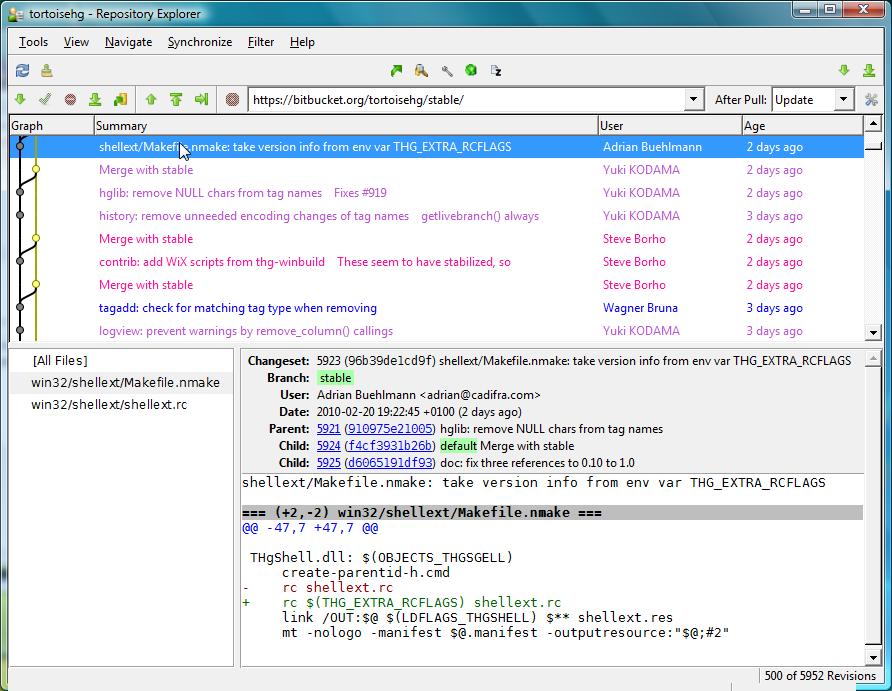
\includegraphics{log.png}
\caption{Changelog viewer dialog with main toolbar hidden}\end{figure}

The changelog tool has a menu bar for accessing tool functions and for
launching other tools.
\begin{quote}
\begin{description}
\item[\textbf{Tools}]
Launch other TortoiseHg tools as separate processes

\item[\textbf{View}]
Toggle the visibility of various features, or refresh views

\item[\textbf{Navigate}]
Select specific changesets in your repository history

\item[\textbf{Synchronize}]
Access synchronization functions, more below

\item[\textbf{Help}]
Help contents shows this web page.  About shows TortoiseHg
version info

\end{description}
\end{quote}

The toolbar buttons from left to right:
\begin{quote}
\begin{description}
\item[\textbf{Refresh}]
Reload the revision history (if you commit in another window, etc)

\item[\textbf{Reset Marks}]
Remove `new', `incoming', and `outgoing' revision marks and refresh

\item[\textbf{Patch Queue}]
Toggles the display of the MQ pane.  This button is only visible
when the MQ extension has been enabled by the user.

\item[\textbf{Commit}]
Launch the commit tool in a separate process

\item[\textbf{Datamine}]
Launch the data mining tool in a separate process

\item[\textbf{Recovery}]
Launch the recovery dialog in a separate process

\item[\textbf{Web Server}]
Launch the web server dialog in a separate process

\item[\textbf{Shelve}]
Launch the shelve tool in a separate process

\item[\textbf{Load more}]
Load the next N revisions into the graph

\item[\textbf{Load all}]
Load all remaining revisions into the graph

\end{description}
\end{quote}


\subsection{Sync Bar}
\begin{figure}[htbp]
\centering


\includegraphics{syncbar.png}
\caption{Synchronization features in changelog tool}\end{figure}

From left to right...
\begin{quote}
\begin{description}
\item[\textbf{Incoming}]
Download incoming changesets from the remote repository, store
them in a temporary bundle file, then enter bundle preview mode
with the incoming changes applied.  Incoming changesets will
have a `down' arrow in the revision graph.

\item[\textbf{Accept}]
Accept (pull) the changesets from the previewed bundle.  This
button is only sensitive when previewing a changeset bundle.
The after-pull effect is respected after pulling from a bundle.

\item[\textbf{Reject}]
Reject the changesets from the previewed bundle and exit preview
mode.  This button is only sensitive when previewing a changeset
bundle.

\item[\textbf{Pull}]
Pull incoming changesets from the remote repository, then apply
after-pull effect (update, fetch, or rebase).

\item[\textbf{Import}]
Open the import dialog to import one or more patches

\item[\textbf{Outgoing}]
Determine outgoing changesets that would be pushed to the
remote repository.  Outgoing changesets are marked with an `up'
arrow.

\item[\textbf{Push}]
Push outgoing changesets to the remote repository.

\item[\textbf{Email}]
Email outgoing changesets to the remote repository.

\item[\textbf{Stop}]
Stop current transaction.  The button is only sensitive during
outgoing commands.

\end{description}
\end{quote}

To the right of the \textbf{Stop} button is a combo box containing
all of the configured peer repository paths for the current repository.
The default path is selected at startup, if it has been configured.
See \href{http://www.selenic.com/mercurial/hg.1.html\#urls}{hg.1.html\#urls}  for
details on specifying remote repository URLs.

To the right of the path combo box is the \textbf{After Pull} combo
that selects the operation which is performed after every pull operation
triggered by the sync bar.  The user must have the rebase extension
enabled in order for that option to be available in the after pull
combo.  The same is true of the fetch extension and it's post pull
operation.

To the right of the \textbf{After Pull} combo is the
\textbf{Settings} button.  It opens the repository settings tool on
the \textbf{Sync} tab where the after pull configurable and peer
repository paths can be configured.

Changesets which are added to the repository after the changelog tool
was opened are marked with green stars in the graph.  This includes
recent commits, pulled changesets, and applied patches.

\begin{notice}{note}{Note:}
To clear the new, incoming, and outgoing marks from the changeset
graph, use \textbf{View -\textgreater{} Reset Marks}
\end{notice}


\subsection{Search Bar}
\begin{figure}[htbp]
\centering


\includegraphics{searchbar.png}
\caption{Filter features in changelog tool}\end{figure}

The search bar allows one to quickly filter the changesets panel.
Buttons from right to left...
\begin{quote}
\begin{description}
\item[\textbf{All}]
Show all changesets in the respository.  Essentially removes all
filters.

\item[\textbf{Tagged}]
Show only changesets with tags.

\item[\textbf{Ancestry}]
Show only changesets that are ancestors of the currently
selected changeset.  This option is only sensitive when a
revision is selected.

\item[\textbf{Parents}]
Show only the working directory parent revisions.  Unless a
merge is in progress, this will be only one revision.

\item[\textbf{Heads}]
Show only repository heads (changesets without any child
revisions).

\item[\textbf{Merges}]
Show only merge changesets (changesets with two parents)

\item[\textbf{Hide Merges}]
A toggle button, not a radio like the other buttons in the
search bar, which toggles the display of merge changesets.

\item[\textbf{Branches}]
A combo box with the list of named branches in your repository.
See \textbf{Repo Settings -\textgreater{} Changelog -\textgreater{} Dead Branches} for
a method to prune names from this combo box.

\item[\textbf{Custom Filter Combo}]
Finally there is a combo box that selects among the various
filter types that can be manually specified.

\end{description}
\end{quote}

To specify a custom filter, the user selects the filter type, enters
the search text of that type, and then hits return in the text entry.
\begin{quote}
\begin{description}
\item[\textbf{Rev Range}]
Parse the user text as a revision range.  See
\href{http://www.selenic.com/mercurial/hg.1.html\#revisions}{hg.1.html\#revisions}
for details on how to specify revision ranges.

\item[\textbf{File Patterns}]
Parse the user text as a file pattern glob, unless the user text
is prefixed with a pattern type like \emph{regexp:}.  See
\href{http://www.selenic.com/mercurial/hg.1.html\#patterns}{hg.1.html\#patterns}
for details on how to specify file patterns.

\item[\textbf{Keywords}]
Parse the user text as a keyword pattern that should be matched
against changeset meta data like comitter, message, etc.

\item[\textbf{Date}]
Parse the user text as a date range.  See
\href{http://www.selenic.com/mercurial/hg.1.html\#dates}{hg.1.html\#dates}
for details on how to specify date ranges.

\item[\textbf{User}]
Parse the user text as a user / comitter name.

\end{description}
\end{quote}

The filter entry has a combo box which stores the history of searches.
Selecting an item from the drop down list will apply that filter.


\subsection{Revision Graph Details}

The graph column shows the child-parent relationships between revisions
in your repository history.  This column auto-sizes for as many lines of
ancestry that are required to visualize the revisions you have loaded.
The column has an initial hard-limit width to prevent some degenerative
cases from breaking the viewer, but can be resized after refreshes.


\subsection{Performance Implications}

There are some Repository Explorer features that should probably be
avoided in large repositories.
\begin{itemize}
\item {} \begin{description}
\item[\emph{View -\textgreater{} Color By Branch}]
This option requires the log viewer to query the branch name of
every revision in order to draw the graph.  It can cause refreshes
to be slow.

\end{description}

\item {} \begin{description}
\item[\emph{View -\textgreater{} Compact Graph}]
This option can cause refresh to be slower than the default setting.
Also be aware that enabling this feature makes the graph lines less
accurate.  The feature trades merge parent accuracy for horizontal
screen space.

\end{description}

\item {} \begin{description}
\item[Column \textbf{Changes}]
This column can be expensive to calculate on repositories with large
working copies, causing both refreshes and scrolling to be slow.

\end{description}

\end{itemize}


\subsection{Revision Context Menus}

Right-clicking on a revision in the (top) graph pane will bring up the
revision context menu.
\begin{quote}
\begin{description}
\item[\textbf{Visualize Change}]
open this change in your visual diff tool

\item[\textbf{Display Change}]
open this changeset in the changeset browser (more below)

\item[\textbf{Diff to Local}]
display changes (visual diff) between this revision and your
current working directory

\item[\textbf{Copy Hash}]
copy current revision's full hash to the clipboard

\item[\textbf{Update...}]
update your working directory to this revision \footnote{
Opens the TortoiseHg update dialog with this revision selected.
}

\item[\textbf{Merge With...}]
merge with this revision \footnote{
Opens the TortoiseHg merge dialog with this revision selected.
}

\item[\textbf{Backout...}]
create a backout changeset for selected revision

\item[\textbf{Revert}]
revert working copy to this revision's contents, without
updating working directory parent revision. Use with care.

\item[\textbf{Export}]\begin{description}
\item[\textbf{Export Patch}]
generate a patch file containing this revision's changes

\item[\textbf{Email Patch}]
send this revision's changes to email recipient \footnote{
Opens the TortoiseHg email dialog with this revision selected.
}

\item[\textbf{Bundle rev:tip}]
create a bundle with all revs from selected to tip

\item[\textbf{Archive...}]
open the archive dialog for this revision, allowing user to
generate a backup copy of the repository at that revision.

\end{description}

\item[\textbf{Tag}]\begin{description}
\item[\textbf{Add/Remove Tag}]
opens the TortoiseHg tag dialog with this revision selected

\item[\textbf{Add/Move/Remove Bookmark}]
opens the TortoiseHg bookmark dialog with this revision selected
\emph{This option requires the boomarks extension to be enabled}

\item[\textbf{Rename Bookmark}]
opens the TortoiseHg bookmark rename dialog
\emph{This option requires the boomarks extension to be enabled}

\end{description}

\item[\textbf{Mercurial Queues}]\begin{description}
\item[\textbf{Import revision to MQ}]
Import selected revision into the current patch queue.  Only
valid for qbase or checked out head revision.  \emph{Only visible
when MQ is enabled}

\item[\textbf{Strip Revision...}]
Remove the selected revision and all of it's descendants from the
repository \footnote{
The strip command will store the stripped revisions in a bundle file
that can later be reapplied.
See \href{http://mercurial.selenic.com/wiki/EditingHistory}{also}.
} \emph{Only visible when MQ is enabled}

\end{description}

\item[\textbf{Transplant to local}]
Transplant selected revision onto the current working parent.
\emph{Only visible when the transplant extension is enabled}

\item[\textbf{Bisect}]\begin{description}
\item[\textbf{Reset}]
Reset bisect state. See \hyperlink{id10}{bisect} section below.

\item[\textbf{Mark as Good}]
Mark changeset as good

\item[\textbf{Mark as Bad}]
Mark changeset as bad

\item[\textbf{Skip Testing}]
Skip testing this changeset

\end{description}

\end{description}
\end{quote}

If you right-click on a row other than the one that was currently
selected, you get a secondary context menu which defines commands that
operation on revision ranges.
\begin{quote}
\begin{description}
\item[\textbf{Diff with selected}]
Opens status viewer with cumulative changes of the range of
changesets.  The status viewer allows cherry picked changes to
be saved to a file.

\item[\textbf{Visual Diff with selected} \footnote{
\emph{Global Settings \(\rightarrow\) TortoiseHg \(\rightarrow\) Visual Diff Tool}
}]
Opens visual diff window with cumulative changes of the range
of changesets.

\item[\textbf{Email from here to selected}]
Opens email dialog with range of changesets.

\item[\textbf{Bundle from here to selected}]
Creates a bundle file with range of changesets.

\item[\textbf{Export patches from here to selected}]
Creates a patch file for each changeset in selected range.

\item[\textbf{Merge with selected} \footnote{
Only sensitive if the selected revision is your current working
directory parent
}]
Merges this revision with the other selected revision.  If
neither revision is currently checked out, the merge dialog will
be forced to update to the first selected revision before
starting the merge.  This will fail if the working directory is
not clean.

\item[\textbf{Transplant revision range to local}]
Transplant selected range of changesets on to current working
parent revision. \emph{Only visible when the transplant extension is
enabled}

\item[\textbf{Rebase on top of selected}]
Rebase selected changeset and ancestors on top of original
selected revision.  \emph{Only visible when the rebase extension is
enabled}

\item[\textbf{qimport from here to selected}]
Import selected revision range into the current patch queue.
\emph{Only visible when MQ is enabled}

\end{description}
\end{quote}


\subsection{File Context Menus}

Right-clicking on filenames in the file list (bottom left) pane will
bring up a context menu for the selected file:
\begin{quote}
\begin{description}
\item[\textbf{Visual Diff}]
Open this revision of the file in your visual diff tool

\item[\textbf{Diff to Local}]
Visualize differences between this revision and your checked
out version

\item[\textbf{View at Revision}]
Open this revision of the file in your visual editor \footnote{
\emph{Global Settings \(\rightarrow\) TortoiseHg \(\rightarrow\) Visual Editor}
}

\item[\textbf{Save at Revision}]
Write this revision of the file to specified location

\item[\textbf{File History}]
Show revisions that modified this file \footnote{
Does not show revisions where a file was deleted, as this is only a
manifest change, it does not modify the file's history.
}

\item[\textbf{Annotate File}]
Open this file in the datamine app, annotated at this revision

\item[\textbf{Revert File Contents}]
Checkout this specific revision of this file \footnote{
The new contents will appear as local changes and must be committed.
}

\end{description}
\end{quote}


\subsection{Changeset browser}

The changeset browser will only show a single file's diffs at a time, as
a performance optimization.  If you would like to see all of the file
diffs at once, click on the \textbf{{[}All Files{]}} row.  The changeset
browser will also skip displaying diffs for files which are above a
maximum limit. See
\emph{Global Settings \(\rightarrow\) TortoiseHg \(\rightarrow\) Max Diff Size}.  The
size limit can be temporarily disabled by toggling \emph{View
-\textgreater{} Ignore Max Diff Size}.

The changelog and datamine tools can open the changeset browser to view
a single revision or the combined effect of a range of revisions. The
changeset browser is very similar to the commit and shelve tools. It has
a file list on the left of all files that have been changed, and a diff
pane on the right with the changes to each file.

The diff pane is tabbed and allows one to select files and hunks that
you wish to extract from the changeset(s) you are browsing and write
them to a patch file using the \textbf{Save as} toolbar button.  This
is a very efficient way to cherry pick changes from a repository.  This
changeset browser also supports the \code{Ctrl-C} keyboard accelerator
to copy hightlighted diff hunks to the clipboard.

Unfortunately, TortoiseHg still does not have a dialog for importing
patches into a repository, so this must be done on the command line with
the \textbf{hg import} command.


\subsection{Message Parsing}

New in TortoiseHg 1.0, the repository browser will detect and underline
changeset hashes, HTTP(s) URLs, and bug report identifiers inside
changeset messages.  These underlined phrases are clickable links.

Every word-boundary delimited string of 12 or 40 characters from the
range {[}0-9a-f{]} is considered a changeset link. Clicking on it in the
repository explorer will jump to the given changeset if possible.

HTTP and HTTPS URLs are similarly turned into clickable links which are
opened in your default web browser.

Issue tracker links are enabled when configured in the tortoisehg
section of your configuration files.  Since only a single issue tracker
can be configured at a time, it is typically configured in the
repository's \code{.hg/hgrc} file.  There are two keys: issue.regex and
issue.link. The first defines the regex to match when picking up issue
numbers, while the second defines the command to run when an issue
number is recognized.

You may include groups in issue.regex, and corresponding \{n\} tokens in
issue.link (where n is a non-negative integer). \{0\} refers to the entire
string matched by issue.regex, while \{1\} refers to the first group and
so on. If no \{n\} tokens are found in issue.link, the entire matched
string is appended instead.

Examples:

\begin{Verbatim}[commandchars=@\[\]]
BitBucket:
issue.regex = @#(\d+)\b
issue.link = http://bitbucket.org/@textless[]your project and repo@textgreater[]/issue/{1}/

Mercurial:
issue.regex = \bissue\d+\b
issue.link = http://mercurial.selenic.com/bts/
\end{Verbatim}


\subsection{Bisect}

TortoiseHg 1.0 introduced support for bisect bug searching to help find
changesets which introduce problems. To use, mark the earliest changeset
you know exhibits the problem as bad, then mark the latest changeset
which is free from the problem as good.  Once you have performed tests,
mark the working directory parent as good or bad, and bisect will either
update to another candidate changeset or announce that it has found the
bad revision.

As a shortcut, you can also mark a revision as good or bad without
checking it out first.

For more automated bisecting, you must use the Mercurial command line
and provide an automated test that can build and run a changeset and
return 0-good, 125-skip, or 127-abort, or anythin else to mean bad.  See
the \textbf{hg bisect} command help for more information.


\subsection{Keyboard navigation}
\begin{description}
\item[\code{Ctrl-P}]
Zoom to the working directory parent revision

\item[\code{Ctrl-D}]
Display visual diffs for selected changeset or file

\item[\code{Ctrl-R}]
Refresh repository contents

\item[\code{Ctrl-G}]
Go to a specific revision

\end{description}


\subsection{Configurables}

The changelog browser has a few configurable options that can be set in
the TortoiseHg Settings dialog on the Changelog tab.
\begin{quote}
\begin{description}
\item[\textbf{Author coloring}]
If true, each author's changeset will be given a unique color

\item[\textbf{Long Summary}]
Concatenate commit message lines until 80 chars are reached

\item[\textbf{Graph batch limit}]
Number of revisions to read in each batch load

\item[\textbf{Copy Hash}]
Copy a revision's changeset id hash to the clipboard when selected
{[}DEPRECATED{]}

\item[\textbf{Dead Branches}]
Comma separated list of branch names that should be ignored
when building a list of branch names for a repository.

\item[\textbf{Branch Colors}]
Space separated list of branch names and colors on the
form branch:\#XXXXXX. Spaces and colons in the branch name must be
escaped using a backslash (\textbackslash{}). Likewise some other characters
can be escaped in this way, e.g. \textbackslash{}u0040 will be decoded to the
@ character, and \textbackslash{}n to a linefeed.

\item[\textbf{Hide Tags}]
Space separated list of tags that will not be shown.  Useful
example: Specify ``qbase qparent qtip'' to hide the standard tags
inserted by the Mercurial Queues Extension.

\item[\textbf{Use Expander}]
Show changeset details within an expander.  When contained
within the expander, the details do not scroll with the
changeset contents.

\end{description}
\end{quote}

The exact colors given to particular users can be configured by adding
lines like these to your \code{Mercurial.ini} file:

\begin{Verbatim}[commandchars=@\[\]]
@PYGZlb[]tortoisehg@PYGZrb[]
authorcolor@PYGbe[.]USERNAME @PYGbe[=] color
\end{Verbatim}

The changelog browser also respects the following settings on the
TortoiseHg tab:
\begin{quote}
\begin{description}
\item[\textbf{Tab Width}]
Number of spaces to expand tabs in diffs

\item[\textbf{Max Diff Size}]
Maximum size of file to be diffed

\item[\textbf{Bottom Diffs}]
Show diffs below file list

\end{description}
\end{quote}


\subsection{From command line}

The changelog viewer can be started from command line

\begin{Verbatim}[commandchars=@\[\]]
hgtk log @PYGZlb[]OPTIONS@PYGZrb[] @PYGZlb[]FILE@PYGZrb[]

aliases: history

changelog viewer

options:

 -l --limit  limit number of changes displayed

use "hgtk -v help log" to show global options
\end{Verbatim}

\resetcurrentobjects
\hypertarget{--doc-datamine}{}

\section{Datamine}
\index{datamine.dialog (module)}
\hypertarget{module-datamine.dialog}{}
\declaremodule[datamine.dialog]{}{datamine.dialog}
\modulesynopsis{Dialog used to search repository history}
The datamine application is used to inspect the revision history of your
repository.  It is a tabbed application that supports two tab types,
\emph{Search} and \emph{Annotate}.


\subsection{Search Tabs}
\begin{figure}[htbp]
\centering

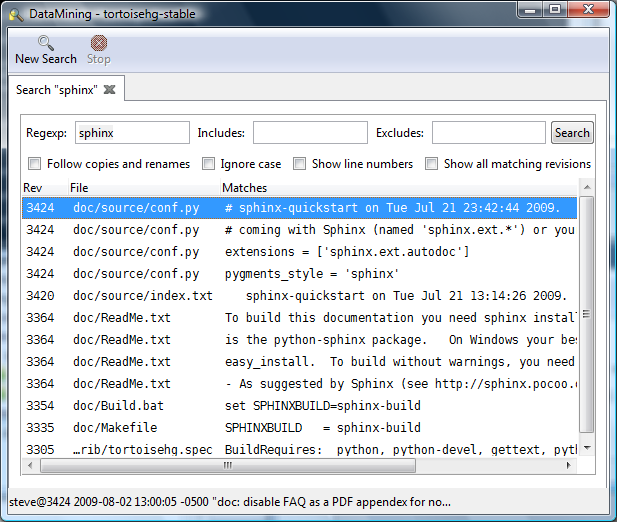
\includegraphics{search.png}
\caption{Search tabs}\end{figure}

The search tab is used to search (\emph{grep}) through your entire revision
history for keywords, variable names, functions, etc...

The text entry fields have these purposes:
\begin{quote}
\begin{description}
\item[\textbf{regexp}]
Regular expression search criteria.

\item[\textbf{includes}]
Comma separated list of paths to include in your search. If no
paths are given, the search is assumed to be repository wide. In
other words, specifying an include path actually narrows the
search criteria.

\item[\textbf{excludes}]
Comma separated list of paths to exclude from your search.
Exclusion patterns are applied after inclusion patterns.

\end{description}
\end{quote}

The toggle buttons below the entry fields are for:
\begin{quote}
\begin{description}
\item[\textbf{Follow copies and renames}]
follow searches through copies and renames out of inclusion filters

\item[\textbf{Ignore case}]
Perform the search without case considerations

\item[\textbf{Show line numbers}]
Show line numbers at the front of the matching lines

\item[\textbf{Show all matching revisions}]
Show every instance where the search criteria matches in a file,
not just the most recent revision.  It shows +/- to indicate
whether the change adds or removes your search text.

\end{description}
\end{quote}

Search tabs are named after the search string most recently used to
start a search.  The \textbf{New Search} toolbar button will
obviously open a new search tab while the \textbf{Stop} button will
terminate an ongoing search (the \textbf{Stop} button is only
sensitive when a search is in progress).


\subsubsection{Matches}

Each match will be a link to a changeset and will have a descriptive
tooltip (author, date/time, summary).  Right clicking on a matched line
will bring up a context menu with these features:
\begin{quote}
\begin{description}
\item[\textbf{display change}]
open a changeset window with this changeset, to see the full context

\item[\textbf{annotate file}]
open an annotation tab for this file at this revision

\item[\textbf{file history}]
open a changelog window with this file's revision history

\item[\textbf{view file at revision}]
open the current file at the specified revision in your favorite
text editor.

\end{description}
\end{quote}


\subsection{Annotate Tabs}
\begin{figure}[htbp]
\centering

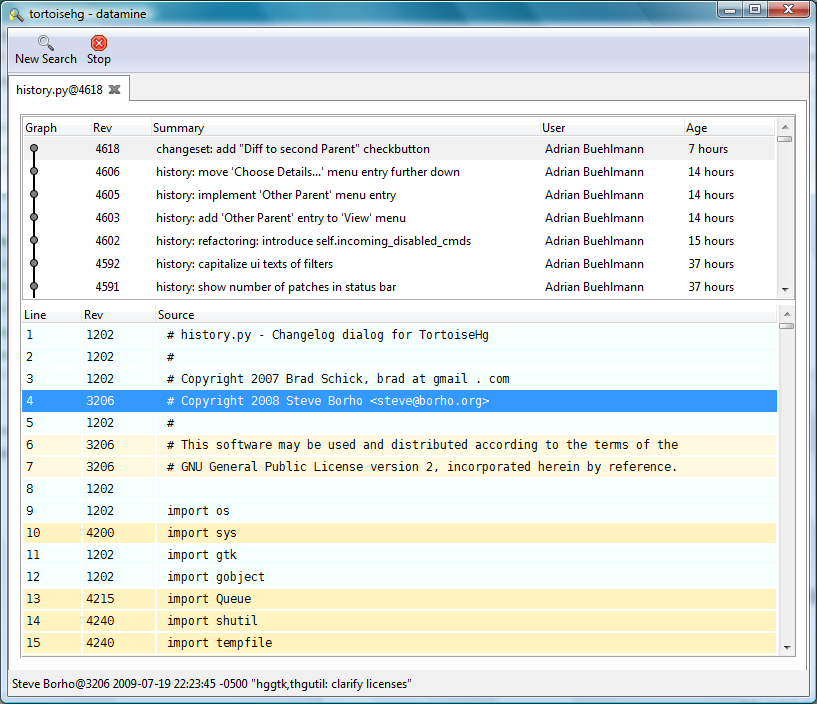
\includegraphics{annotate.png}
\caption{Annotate tabs}\end{figure}

The revision graph has a simple context menu for opening the entire
changeset in the changeset browser. Activating a row in the revision
graph updates the file annotation to that revision.

In the bottom pane is the actual annotation. Each line in the annotation
is also a link to the changeset which provided that line. Activating a
row will zoom the changelog (top pane) to the changeset that introduced
that line and change focus to the top pane.

The color scheme in the annotation pane is two dimensional. Authors
determine hue, and age determines saturation. The older a change, the
lighter the color.

By right-clicking on the annotate pane's column headers (Line, Rev,
Source) you can bring up a menu for showing two optional columns:
\textbf{filename} and \textbf{user}.


\subsubsection{Following Renames}

The annotation data will automatically follow lines of code back through
copies and renames to find the initial changeset that introduced the
line.  The graph log pane will also attempt to follow renames and
copies, so some lines in the graph may correlate to different filenames
than the original annotated file path.  Renames are indicated in the
graph by color changes within a column.


\subsubsection{Configurables}

The annotate tabs support the following configurations defined primarily
for other tools:
\begin{description}
\item[\emph{Changelog \(\rightarrow\) Author Coloring}]
Give each author a separate color in the changelog graph

\item[\emph{Changelog \(\rightarrow\) Long Summary}]
Concatenates lines of commit message together to reach an 80
character summary.

\item[\emph{TortoiseHg \(\rightarrow\) Tab width}]
Number of spaces to expand tabs in diffs and annotate output

\end{description}


\subsection{From command line}

The datamine tool can be started from command line

\begin{Verbatim}[commandchars=@\[\]]
hgtk datamine

aliases: annotate, blame

repository search and annotate tool

use "hgtk -v help datamine" to show global options
\end{Verbatim}

\resetcurrentobjects
\hypertarget{--doc-synchronize}{}

\section{Synchronize}
\index{synchronize.dialog (module)}
\hypertarget{module-synchronize.dialog}{}
\declaremodule[synchronize.dialog]{}{synchronize.dialog}
\modulesynopsis{Dialog used to perform synchronization operations}\begin{figure}[htbp]
\centering

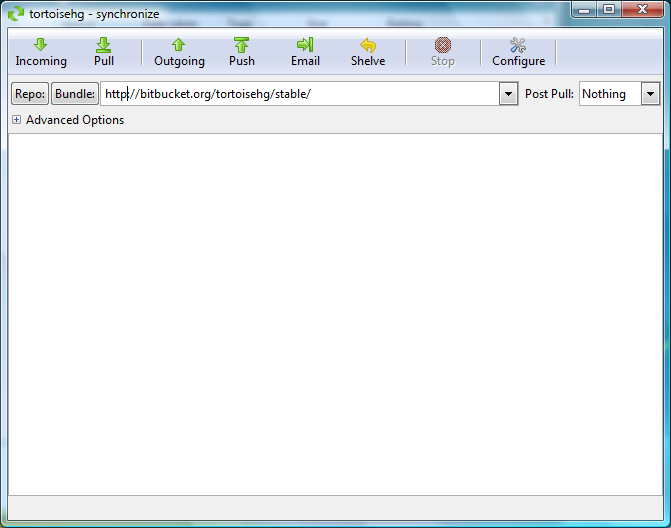
\includegraphics{synchronize.png}
\caption{Synchronize dialog}\end{figure}

\begin{notice}{note}{Note:}
The synchronize tool has been deprecated in the 0.9 release, and may
be removed in a future release.  We suggest you use the changelog
tool for performing synchronization duties.
\end{notice}

The synchronize tool is used to transmit changesets between repositories
or to email recipients.
\begin{quote}
\begin{description}
\item[\textbf{Incoming}]
show changesets that would be pulled from target repository, the
changes in the target repository that are not in local repository

\item[\textbf{Pull}]
pull incoming changesets from target repository

\item[\textbf{Outgoing}]
show changesets that would be pushed to target repository, the
changes in the local repository that are not in target
repository

\item[\textbf{Push}]
push outgoing changesets to target repository, make the local
\emph{tip} the new \emph{tip} in the target repository

\item[\textbf{Email}]
send outgoing changesets (to target repository) as email

\item[\textbf{Shelve}]
launch the shelve tool to allow working changes to be
temporarily moved into the shelf, since some operations require
the working directory to be clean.

\item[\textbf{Stop}]
stop current operation

\item[\textbf{Configure}]
configure repository paths (aliases)

\end{description}
\end{quote}

Below the toolbar are two buttons and a text entry:
\begin{quote}
\begin{description}
\item[\textbf{Repo:}]
browse for a local repository to synchronize with

\item[\textbf{Bundle:}]
browse for a local bundle file to pull from

\end{description}
\end{quote}

The text entry/combo box is where you enter or select paths of target
repositories. The synchronize tool will seed the drop-down list with
path aliases configured for this repository.

The \textbf{Post Pull Operation} frame contains radio buttons for
selecting the operation which is performed after a pull.  This behavior
is configurable via the \textbf{Configure} button.  You can select a
default behavior for your user account and override that selection on a
per-repository basis.
\begin{quote}
\begin{description}
\item[\textbf{Nothing}]
No operations are performed after a pull.  You will be allowed to
view the pulled changesets in the log viewer, and you will have the
option to update to the new tip if applicable.

\item[\textbf{Update}]
Automatically update to the new branch tip if, and only if, new
revisions were pulled into the local repository.  This could trigger
a merge if the pulled changes conflict with local uncommitted
changes.

\item[\textbf{Fetch}]
Equivalent to hg fetch.  See the fetch extension documentation for
it's behavior.  This feature is only available if the fetch
extension has been enabled by the user.

\item[\textbf{Rebase}]
Equivalent to pull --rebase.  See the rebase extension
documentation for it's behavior.  This feature is only available
if the rebase extension has been enabled by the user.

\end{description}
\end{quote}

The \textbf{use proxy} button is a quick way to disable your proxy
configuration for individual operations. The button is only sensitive
when an http proxy is configured.

All operations which require authentication will pop up dialog boxes to
get the required information from the user.  TortoiseHg uses the
TortoisePlink tool (borrowed from the TortoiseSVN distribution) to
handle \emph{ssh:} connections and authentication.  See the \href{http://bitbucket.org/tortoisehg/stable/wiki/FAQ\#tortoisehg-faq}{FAQ} for help if
you have trouble connecting to ssh servers.

Under the \textbf{Advanced Options} fold-up panel are a number of
configurables that are valid for most push/pull operations.
\begin{quote}
\begin{description}
\item[\textbf{Force pull or push}]
override warnings about multiple heads or unrelated repositories

\item[\textbf{Target Revision}]
to avoid sending all revisions

\item[\textbf{Remote Command}]
provides -e argument

\item[\textbf{Show patches}]
show diffs in incoming and outging changes

\item[\textbf{Show Newest First}]
reverse order that changesets are listed

\item[\textbf{Show No Merges}]
filter out merge changesets from output (does not affect push/pull)

\end{description}
\end{quote}


\subsection{After Pull}

After changesets are pulled into your repository, a buttons may appear
at the bottom of the dialog:
\begin{quote}
\begin{description}
\item[\textbf{Update to branch tip}]
Update your working directory to the new tip of the current branch

\end{description}
\end{quote}

The button will be hidden when it is not applicable.


\subsection{Email}
\begin{figure}[htbp]
\centering

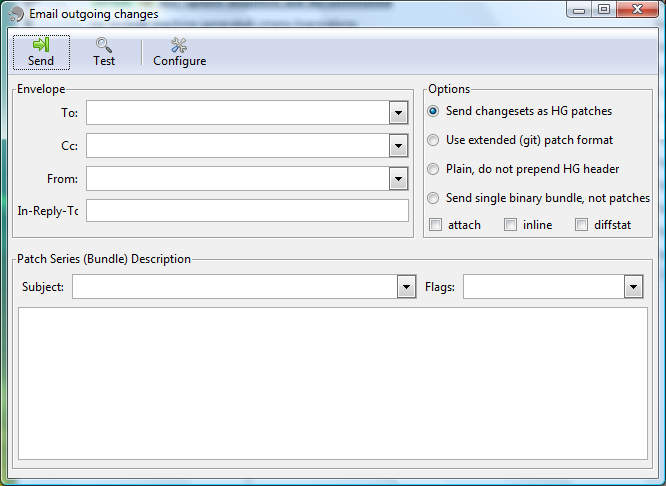
\includegraphics{email.png}
\caption{Email dialog}\end{figure}

The email dialog can be launched from two TortoiseHg tools.
\begin{enumerate}
\item {} 
The changelog tool, in which case the user intends to email a single
revision or a range of revisions.

\item {} 
The synchronize tool, in which case the user intends to email all
outgoing changes to the current target repository (it's good practice to
check the outgoing changes before launching the email dialog).

\end{enumerate}

The \textbf{Send} button is obvious, and the \textbf{Configure}
dialog predictably opens the TortoiseHg Settings dialog to the email tab
where you can configure your SMTP settings and set default
\textbf{To:} and \textbf{From:} addresses.

\textbf{In-Reply-To:} is used to make your patches properly threaded
in mailing lists.

Please consult the Mercurial documentation for the differences between
plain patches, Hg patches, Git patches, and bundles.


\subsection{From command line}

The synchronize tool can be started from command line

\begin{Verbatim}[commandchars=@\[\]]
hgtk synch

aliases: pull, push, incoming, outgoing, email

repository synchronization tool

use "hgtk -v help synch" to show global options
\end{Verbatim}

The syntax is simple, no options or parameters are needed, except the
global options.  If the synchronize tool is started via push, outgoing,
or email command aliases, it will automatically select the
\emph{default-push} URL if.  For all other aliases the tool selects the
\emph{default} URL.  If the selected URL is not found, it will use the first
path it finds.

\resetcurrentobjects
\hypertarget{--doc-serve}{}

\section{Serve}
\index{serve.dialog (module)}
\hypertarget{module-serve.dialog}{}
\declaremodule[serve.dialog]{}{serve.dialog}
\modulesynopsis{Dialog used to start/stop the web server}\begin{figure}[htbp]
\centering

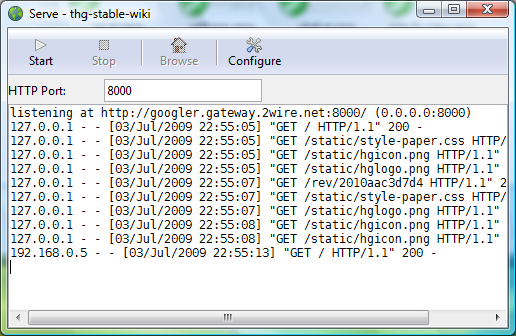
\includegraphics{serve.png}
\end{figure}

The serve tool is a wrapper for Mercurial's built-in web server. Once
launched, any computer can attach to the http port and browse your
repository(ies) or perform clone, pull, or even push operations (if you
configure your server to allow it).

Toolbar buttons:
\begin{quote}
\begin{description}
\item[\textbf{Start}]
start the web server

\item[\textbf{Stop}]
stop the web server

\item[\textbf{Browse}]
open your default browser at the built-in web server

\item[\textbf{Configure}]
Configure repository web style, description, and access policies

\end{description}
\end{quote}

When the settings dialog is launched via the \textbf{Configure}
button, it is run in the context of the current repository.  Please
visit the Mercurial wiki for detailed descriptions of the various
web configurations.


\subsection{Multiple Repositories}

If you wish to serve a many repositories with a single web server
instance, you can create an \code{hgwebdir.conf} text file with the
following contents:

\begin{Verbatim}[commandchars=@\[\]]
@PYGZlb[]paths@PYGZrb[]
/ = /path/to/repositories/*
\end{Verbatim}

The first path `/' is where the repositories will appear in the context
of the web server and the second path describes here the repositories
can be found on your computer.  Multiple entries are possible.

To use this file you must launch the TortoiseHg serve dialog from the
command line via: \textbf{hgtk serve --webdir-conf=hgwebdir.conf}.


\subsection{From command line}

The server tool can be started from command line

\begin{Verbatim}[commandchars=@\[\]]
hgtk serve @PYGZlb[]OPTION@PYGZrb[]...

web server

options:

        --webdir-conf  name of the webdir config file

use "hgtk -v help serve" to show global options
\end{Verbatim}

\resetcurrentobjects
\hypertarget{--doc-guess}{}

\section{Rename Guessing}
\index{guess.dialog (module)}
\hypertarget{module-guess.dialog}{}
\declaremodule[guess.dialog]{}{guess.dialog}
\modulesynopsis{Dialog used to detect copies and/or renames}\begin{figure}[htbp]
\centering

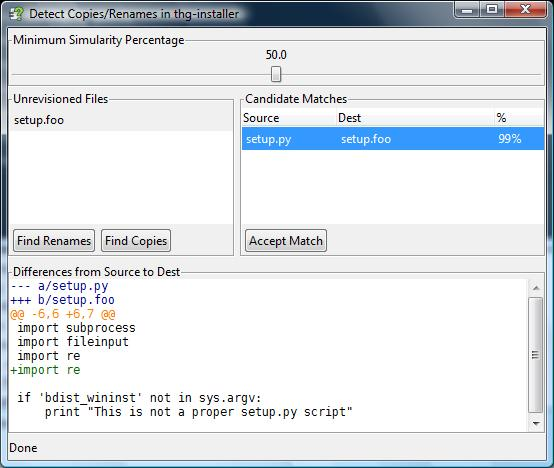
\includegraphics{guess.jpg}
\caption{Rename Guessing Dialog}\end{figure}

This dialog is used to find renames, moves, and/or copies that were done
without Mercurial's knowledge.  The dialog can be launched from the
shell context menu, or from the status or commit tools via the context
menu of an unknown file.

Follow these steps:
\begin{enumerate}
\item {} 
select one or more of the \textbf{Unrevisioned Files}

\item {} 
slide the simularity bar to the percentage match you desire

\item {} 
press either \textbf{Find Renames} or \textbf{Find Copies}.

\item {} 
select candidate matches and accept good matches

\item {} 
repeat until all unrevisioned files are matched

\end{enumerate}


\subsection{Find Renames}

This feature will search the repository for missing files (files which
were revisioned but are now gone).  For each missing file, it compares
the last revisioned data against the unrevisioned file and if the
percentage of matching lines is above the
\textbf{Minimum Simularity Percentage}, it adds the pair to the
\textbf{Candidate Matches}.


\subsection{Find Copies}

This feature will check every revisioned file in the repository to see
if it exactly matches the unrevisioned file.


\subsection{Candidate Matches}

When you select a match in this list, the differences between the two
files are shown in the bottom pane.  Pressing \textbf{Accept Match}
will record the rename or copy event with Mercurial.


\subsection{From command line}

The guess tool can be started from command line:

\begin{Verbatim}[commandchars=@\[\]]
hgtk guess

guess previous renames or copies

use "hgtk -v help guess" to show global options
\end{Verbatim}

\resetcurrentobjects
\hypertarget{--doc-ignore}{}

\section{Ignore Filter}
\index{ignore.dialog (module)}
\hypertarget{module-ignore.dialog}{}
\declaremodule[ignore.dialog]{}{ignore.dialog}
\modulesynopsis{Dialog used to maintain the ignore filter}
The ignore dialog is used to maintain your Mercurial repository's ignore
filter, which can be found in an \code{.hgignore} file in the
repository root.  The dialog can be launched from the shell context
menu, or from the status or commit tools via the context menu of an
unknown file.
\begin{figure}[htbp]
\centering

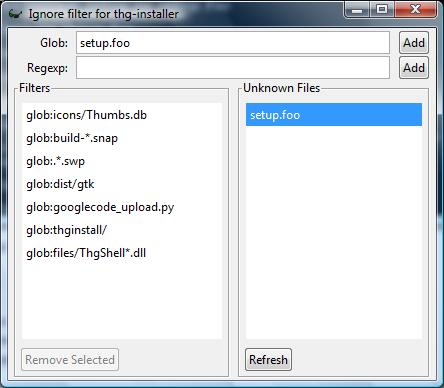
\includegraphics{ignore.jpg}
\caption{Ignore Filter Dialog}\end{figure}


\subsection{From command line}

The ignore tool can be started from command line:

\begin{Verbatim}[commandchars=@\[\]]
hgtk hgignore @PYGZlb[]FILE@PYGZrb[]

aliases: ignore, filter

ignore filter editor

use "hgtk -v help hgignore" to show global options
\end{Verbatim}

\resetcurrentobjects
\hypertarget{--doc-settings}{}

\chapter{Settings}
\index{settings.dialog (module)}
\hypertarget{module-settings.dialog}{}
\declaremodule[settings.dialog]{}{settings.dialog}
\modulesynopsis{Dialog used to set preferences}\begin{figure}[htbp]
\centering

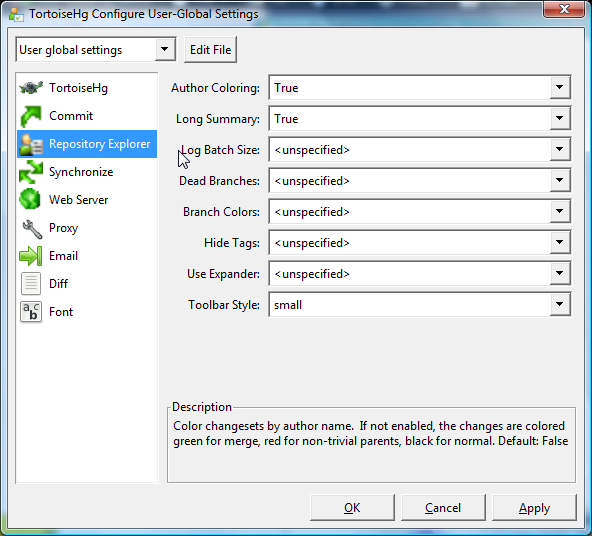
\includegraphics{settings.png}
\caption{Settings dialog}\end{figure}

The Settings dialog is used to configure both TortoiseHg and the
underlying Mercurial DVCS.  Since TortoiseHg uses Mercurial's underlying
configuration system to store and retrieve its settings, these are
essentially the same thing.

Mercurial on Windows has a three-tier configuration system.
\begin{enumerate}
\item {} 
A site-wide configuration file in
\code{C:\textbackslash{}Program Files\textbackslash{}TortoiseHg\textbackslash{}Mercurial.ini}
This file is read first and thus has the lowest priority.

\item {} 
A per-user configuration file in
\code{C:\textbackslash{}Documents and Settings\textbackslash{}username\textbackslash{}Mercurial.ini}
This file is read second and thus can override settings in the
site-wide configuration file.

\item {} 
A per-repository configuration file in \code{repo-root\textbackslash{}.hg\textbackslash{}hgrc} This
file is read last and can override site-wide and user global settings.

\end{enumerate}

The site-wide file can be overwritten on upgrades so it is recommended
that you do not make changes to this file.  Instead, you should make
changes to your user \code{Mercurial.ini} and/or the repository
\code{hgrc} file.  The TortoiseHg Settings dialog enforces this
suggestion by only operating in two modes:
\begin{description}
\item[Global]
edits your user \code{Mercurial.ini} file

\item[Repository]
edits a repository \code{.hg/hgrc} file

\end{description}

You may toggle between the two modes using the combo box at the top of
the dialog, or directly edit the file in your configured visual editor.

Most TortoiseHg users will want to store all configurables in their
global user settings, and only use the repository hgrc to store paths
(remote repository aliases) and web settings, though it is possible to
override many configurables per-repository (a common example is to
configure a username for use in a specific repository).  Also note that
the user and repository configuration files may not exist until you run
the Settings dialog for the first time.


\section{Tabs}

The Settings tool is a tabbed application.

Each tab corresponds roughly to a section of your \code{Mercurial.ini}
file, though there is a certain amount of overlap. Some sections were
split across multiple tabs for clarity.

Every tab but \textbf{Sync} has the same format, a list of
configurable options with a drop-down combo box with possible values and
a history of options you have used for that setting. The configurable
name (label) has a tooltip which describes in more detail what you are
configuring and its default value.  The description of the currently
focused configurable is also shown in a text box at the bottom of the
dialog.

Please consult the Mercurial wiki for more detailed information about
these configurables (except for the first three tabs:
\textbf{TortoiseHg}, \textbf{Commit}, \textbf{Changelog}, which
are specific to TortoiseHg).
\index{TortoiseHg.settings (module)}
\hypertarget{module-TortoiseHg.settings}{}
\declaremodule[TortoiseHg.settings]{}{TortoiseHg.settings}
\modulesynopsis{Dialog used to set general TortoiseHg preferences}

\subsection{TortoiseHg}
\begin{description}
\item[\textbf{3-way Merge Tool:}]
Graphical merge program for resolving merge conflicts.  If left
unspecified, Mercurial will use the first applicable tool it finds
on your system or use its internal merge tool that leaves conflict
markers in place.  Chose \textbf{internal:merge} to force
conflict markers, \textbf{internal:prompt} to always select local
or other, or \textbf{internal:dump} to leave files in the working
directory for manual merging.

\item[\textbf{Visual Diff Tool:}]
Specify visual diff tool as described in the {[}merge-tools{]} section
of your Mercurial configuration files.  If left unspecified,
TortoiseHg will use the selected merge tool. Failing that it uses
the first applicable tool it finds.

\item[\textbf{Skip Diff Window:}]
Bypass the builtin visual diff dialog and directly use your
visual diff tool's directory diff feature.  Only enable this
feature if you know your diff tool has a valid extdiff
configuration.  Default: False.

\item[\textbf{Visual Editor:}]
Specify the visual editor used to view files, etc.

\item[\textbf{CLI Editor:}]
The editor to use during a commit and other
instances where Mercurial needs multiline input from
the user.  Only used by command line interface commands.

\item[\textbf{Tab Width:}]
Specify the number of spaces that tabs expand to in various
TortoiseHg windows. Default: Not expanded.

\item[\textbf{Max Diff Size:}]
The maximum size file (in KB) that TortoiseHg will
show changes for in the changelog, status, and commit windows.
A value of zero implies no limit.  Default: 1024 (1MB).

\item[\textbf{Bottom Diffs:}]
Show the diff panel below the file list in status, shelve, and
commit dialogs.  Default: False (show diffs to right of file list).

\item[\textbf{Capture stderr:}]
Redirect stderr to a buffer which is parsed at the end of the process
for runtime errors. Default: True.

\item[\textbf{Fork hgtk:}]
When running hgtk from the command line, fork a background process
to run graphical dialogs. Default: True.

\item[\textbf{Full Path Title:}]
Show a full directory path of the repository in the dialog title
instead of just the root directory name.  Default: False

\item[\textbf{Spell Check Language:}]
Default language for spell check.  System language is used if not
specified.  Examples: en, en\_GB, en\_US.  Spell checking requires
gtkspell, which is only available on Gnome PCs.

\end{description}
\index{commit.settings (module)}
\hypertarget{module-commit.settings}{}
\declaremodule[commit.settings]{}{commit.settings}
\modulesynopsis{Dialog used to set commit specific preferences}

\subsection{Commit}
\begin{description}
\item[\textbf{Username:}]
Name associated with commits.

\item[\textbf{Summary Line Length:}]
Maximum length of the commit message summary line.
If set, TortoiseHg will issue a warning if the
summary line is too long or not separated by a
blank line. Default: 0 (unenforced).

\item[\textbf{Message Line Length:}]
Word wrap length of the commit message.  If
set, the popup menu can be used to format
the message and a warning will be issued
if any lines are too long at commit.
Default: 0 (unenforced).

\item[\textbf{Push After Commit:}]
Attempt to push to default push target after every successful
commit.  Default: False

\item[\textbf{Auto Commit List:}]
Comma separated list of files that are automatically included in
every commit.  Intended for use only as a repository setting.
Default: None

\item[\textbf{Auto Exclude List:}]
Comma separated list of files that are automatically unchecked when
the status, commit, and shelve dialogs are opened.  Default: None

\end{description}
\index{changelog.settings (module)}
\hypertarget{module-changelog.settings}{}
\declaremodule[changelog.settings]{}{changelog.settings}
\modulesynopsis{Dialog used to set changelog specific preferences}

\subsection{Changelog}
\begin{description}
\item[\textbf{Author Coloring:}]
Color changesets by author name.  If not enabled,
the changes are colored green for merge, red for
non-trivial parents, black for normal.
Default: False.

\item[\textbf{Long Summary:}]
If true, concatenate multiple lines of changeset summary
until they reach 80 characters.
Default: False.

\item[\textbf{Log Batch Size:}]
The number of revisions to read and display in the
changelog viewer in a single batch.
Default: 500.

\item[\textbf{Dead Branches:}]
Comma separated list of branch names that should be ignored when
building a list of branch names for a repository.  Default: None

\item[\textbf{Branch Colors:}]
Space separated list of branch names and colors of the form
branch:\#XXXXXX. Spaces and colons in the branch name must be escaped
using a backslash (\textbackslash{}). Likewise some other characters can be
escaped in this way, e.g. \textbackslash{}u0040 will be decoded to the @
character, and \textbackslash{}n to a linefeed.  Default: None

\item[\textbf{Hide Tags:}]
Space separated list of tags that will not be shown.
Useful example: Specify ``qbase qparent qtip'' to hide the
standard tags inserted by the Mercurial Queues Extension.
Default: None.

\end{description}
\index{synchronize.settings (module)}
\hypertarget{module-synchronize.settings}{}
\declaremodule[synchronize.settings]{}{synchronize.settings}
\modulesynopsis{Dialog used to set synchronize specific preferences}

\subsection{Sync}

The \textbf{Sync} tab is where you can store URLs (paths) to related
repositories. It is rare to store paths in the site-wide or user
configuration files, most of the time you will only store these in a
repository configuration file. Mercurial has two special path names that
can be used as default targets for some operations.
\begin{itemize}
\item {} 
\emph{default}     - the default URL to pull from, usually clone source

\item {} 
\emph{default-push} - the default push target when using the command line

\end{itemize}
\begin{description}
\item[\textbf{After Pull Operation:}]
Operation which is performed directly after a successful pull.
\textbf{update} equates to \textbf{pull --update}, \textbf{fetch}
equates to the fetch extension, \textbf{rebase} equates to
\textbf{pull --rebase}.  Default: none.

\item[\textbf{Remote repository paths}]
In this pane you can configure aliases for repositories that you
frequently synchronize with.  Mercurial will add a \emph{default} alias
to the clone source automatically.  All configured path aliases will
be listed in the Synchronize tool path drop-down box, and they can
be used as short-cuts on the command line.

\end{description}
\index{web.settings (module)}
\hypertarget{module-web.settings}{}
\declaremodule[web.settings]{}{web.settings}
\modulesynopsis{Dialog used to set web server specific preferences}

\subsection{Web}
\begin{description}
\item[\textbf{Name:}]
Repository name to use in the web interface.
Default is the working directory.

\item[\textbf{Description:}]
Textual description of the repository's purpose or
contents.

\item[\textbf{Contact:}]
Name or email address of the person in charge of the
repository.

\item[\textbf{Style:}]
Which template map style to use.

\item[\textbf{Archive Formats:}]
Comma separated list of archive formats allowed for
downloading.

\item[\textbf{Port:}]
Port to listen on.

\item[\textbf{Push Requires SSL:}]
Whether to require that inbound pushes be transported
over SSL to prevent password sniffing.

\item[\textbf{Stripes:}]
How many lines a ``zebra stripe'' should span in multiline output.
Default is 1; set to 0 to disable.

\item[\textbf{Max Files:}]
Maximum number of files to list per changeset.

\item[\textbf{Max Changes:}]
Maximum number of changes to list on the changelog.

\item[\textbf{Allow Push:}]
Whether to allow pushing to the repository. If empty or not
set, push is not allowed. If the special value ``*'', any remote
user can push, including unauthenticated users. Otherwise, the
remote user must have been authenticated, and the authenticated
user name must be present in this list (separated by whitespace
or ``,''). The contents of the allow\_push list are examined after
the deny\_push list.

\item[\textbf{Deny Push:}]
Whether to deny pushing to the repository. If empty or not set,
push is not denied. If the special value ``*'', all remote users
are denied push. Otherwise, unauthenticated users are all
denied, and any authenticated user name present in this list
(separated by whitespace or ``,'') is also denied. The contents
of the deny\_push list are examined before the allow\_push list.

\item[\textbf{Encoding:}]
Character encoding name.

\end{description}
\index{proxy.settings (module)}
\hypertarget{module-proxy.settings}{}
\declaremodule[proxy.settings]{}{proxy.settings}
\modulesynopsis{Dialog used to set proxy specific preferences}

\subsection{Proxy}
\begin{description}
\item[\textbf{Host:}]
Host name and (optional) port of proxy server, for
example \code{myproxy:8000}.

\item[\textbf{Bypass List:}]
Optional. Comma-separated list of host names that
should bypass the proxy.

\item[\textbf{User:}]
Optional. User name to authenticate with at the
proxy server.

\item[\textbf{Password:}]
Optional. Password to authenticate with at the
proxy server.

\end{description}
\index{email.settings (module)}
\hypertarget{module-email.settings}{}
\declaremodule[email.settings]{}{email.settings}
\modulesynopsis{Dialog used to set email specific preferences}

\subsection{Email}
\begin{description}
\item[\textbf{From:}]
Email address to use in the ``From'' header and for the SMTP envelope.

\item[\textbf{To:}]
Comma-separated list of recipient email addresses.

\item[\textbf{Cc:}]
Comma-separated list of carbon copy recipient email
addresses.

\item[\textbf{Bcc:}]
Comma-separated list of blind carbon copy recipient
email addresses.

\item[\textbf{method:}]
Optional. Method to use to send email messages. If value is ``smtp'' (default),
use SMTP (configured below).  Otherwise, use as name of program to run that
acts like sendmail (takes \textbf{-f} option for sender, list of recipients on
command line, message on stdin). Normally, setting this to \code{sendmail} or
\code{/usr/sbin/sendmail} is enough to use sendmail to send messages.

\item[\textbf{SMTP Host:}]
Host name of mail server.

\item[\textbf{SMTP Port:}]
Port to connect to on mail server.
Default: 25.

\item[\textbf{SMTP TLS:}]
Connect to mail server using TLS.
Default: False.

\item[\textbf{SMTP Username:}]
Username to authenticate to mail server with.

\item[\textbf{SMTP Password:}]
Password to authenticate to mail server with.

\item[\textbf{Local Hostname:}]
Hostname the sender can use to identify itself to the mail server.

\end{description}
\index{diff.settings (module)}
\hypertarget{module-diff.settings}{}
\declaremodule[diff.settings]{}{diff.settings}
\modulesynopsis{Dialog used to set diff specific preferences}

\subsection{Diff}
\begin{description}
\item[\textbf{Patch EOL:}]
Normalize file line endings during and after patch to lf or crlf.
Strict does no normalization.  Default: strict

\item[\textbf{Git Format:}]
Use git extended diff header format.
Default: False.

\item[\textbf{No Dates:}]
Do not include modification dates in diff headers.
Default: False.

\item[\textbf{Show Function:}]
Show which function each change is in.
Default: False.

\item[\textbf{Ignore White Space:}]
Ignore white space when comparing lines.
Default: False.

\item[\textbf{Ignore WS Amount:}]
Ignore changes in the amount of white space.
Default: False.

\item[\textbf{Ignore Blank Lines:}]
Ignore changes whose lines are all blank.
Default: False.

\item[\textbf{Coloring Style:}]
Adjust the coloring style of diff lines in the changeset viewer.
Default: foreground.

\end{description}
\index{font.settings (module)}
\hypertarget{module-font.settings}{}
\declaremodule[font.settings]{}{font.settings}
\modulesynopsis{Dialog used to set font specific preferences}

\subsection{Font}
\begin{description}
\item[\textbf{Theme default fonts}]
Use default fonts based on current GTK theme.

\item[\textbf{Preset fonts:}]
Select preset fonts from drop-down combo.  These font sets are tuned
specifically for each language and/or environment.

\item[\textbf{Custom fonts:}]
Set font names and sizes individually for each usage place.

\end{description}

The group which contains drop-down combo entries under
\textbf{Custom fonts:} radio button is enabled when you activate it.
\begin{description}
\item[\textbf{Commit Message:}]
Font used in changeset viewer and commit log text.
Default: monospace 10.

\item[\textbf{Diff Text:}]
Font used for diffs in status and commit tools.
Default: monospace 10.

\item[\textbf{File List:}]
Font used in file lists in status and commit tools.
Default: sans 9.

\item[\textbf{Command Output:}]
Font used in command output window.
Default: monospace 10.

\end{description}


\section{Removed this release}
\begin{description}
\item[\textbf{Copy Hash:}]
Allow the changelog viewer to copy the changeset hash
of the currently selected changeset into the clipboard.
Default: False.

\end{description}

To copy the hash of a changeset to the clipboard, use the `Copy Hash'
context menu option.


\section{Keyboard navigation}
\begin{description}
\item[\code{Ctrl-Enter}]
Apply changes and close the tool, the equivalent of pressing the
`Ok' button.

\end{description}


\section{From command line}

The setting dialog can be started from command line

\begin{Verbatim}[commandchars=@\[\]]
hgtk repoconfig
\end{Verbatim}

for the repository settings (\code{.hg/hgrc} file) or

\begin{Verbatim}[commandchars=@\[\]]
hgtk userconfig
\end{Verbatim}

for the user configuration (\code{Mercurial.ini} file).

The syntax is simple, no options or parameters are needed, except the global
options.

\resetcurrentobjects
\hypertarget{--doc-recovery}{}

\chapter{Recovery}
\index{recovery.dialog (module)}
\hypertarget{module-recovery.dialog}{}
\declaremodule[recovery.dialog]{}{recovery.dialog}
\modulesynopsis{Dialog used to perform recovery operations}\begin{figure}[htbp]
\centering

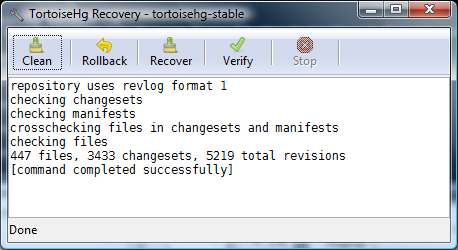
\includegraphics{recover.png}
\caption{Recovery Dialog}\end{figure}

The toolbar buttons equate to a Mercurial command
\begin{description}
\item[\textbf{clean}]
\textbf{hg update --clean} - performs a clean checkout of the
current (first) working directory parent revision.  Undoes an
aborted or partially completed merge.  This will destroy all
changes, please use carefully.  You should shelve any changes you
wish to keep before using this command.

\item[\textbf{rollback}]
\textbf{hg rollback} - undo operation for the most recent
repository transaction, which is usually a commit or a pull.  There
is no way to know for certain what operation will be rolled back, so
only use this in situations where you know what the last transaction
was.

\item[\textbf{recover}]
\textbf{hg recover} - recover from a badly aborted transaction.
This is rarely necessary, and Mercurial will inform you if it ever
needs to be performed.

\item[\textbf{verify}]
\textbf{hg verify} - perform a consistency check of the contents of your
repository.  Completely safe.

\end{description}

\resetcurrentobjects
\hypertarget{--doc-patches}{}

\chapter{Patches}
\index{patches (module)}
\hypertarget{module-patches}{}
\declaremodule[patches]{}{patches}
\modulesynopsis{Describe patch operations}

\section{Defining a patch}

These links are recommended reading for understanding the history and nature
of patches and how they can be used with Mercurial.
\begin{itemize}
\item {} 
\href{http://tortoisehg.bitbucket.org/hgbook/1.4/managing-change-with-mercurial-queues.html\#sec:mq:patch-mgmt}{The patch management problem}

\item {} 
\href{http://tortoisehg.bitbucket.org/hgbook/1.4/managing-change-with-mercurial-queues.html\#sec:mq:patch}{Understanding patches}

\item {} 
\href{http://tortoisehg.bitbucket.org/hgbook/1.4/managing-change-with-mercurial-queues.html\#sec:mq:adv-patch}{More about patches}

\end{itemize}


\section{Pitfalls}

The standard patch format cannot describe binary files, renames, copies,
or permission changes.  If your patch needs to record any of those
things, you will need to enable \textbf{git} patches via:

\begin{Verbatim}[commandchars=@\[\]]
@PYGZlb[]diff@PYGZrb[]
git@PYGbe[=]@PYGaA[True]
\end{Verbatim}

Mercurial 1.5 improves it's behavior in this regard.  It will warn you
when git diffs are required, or sometimes upgrade to the git format
automatically.  See also the
\href{http://www.selenic.com/mercurial/hgrc.5.html\#diff}{diff section} of
the hgrc documentation.

Mercurial's patch routines do not deal well with mixed EOLN between
source files and patches.  The \textbf{patch.eol} setting was introduced in
1.3 to improve this situation:

\begin{Verbatim}[commandchars=@\[\]]
@PYGZlb[]patch@PYGZrb[]
eol @PYGbe[=] auto @PYGaE[@#strict, lf, or crlf]
\end{Verbatim}

The work on the hgeol extension is also improving this area.  Perhaps it
will be resolved by hg-1.5.  See also the
\href{http://www.selenic.com/mercurial/hgrc.5.html\#patch}{patch section}
of the hgrc documentation.

Applying a patch is not a foolproof operation.  If the source file has
diverged from the file that was used to create the patch, there may be
conflicts during the patch application.  These are written to a file
with an .rej extension.  TortoiseHg 1.0 includes an experimental
\textbf{hgtk mpatch} command that can try \emph{harder} to apply the
rejected patch hunks.  This command is based on Chris Mason's \href{http://oss.oracle.com/~mason/mpatch/}{mpatch} utility.  If mpatch cannot
apply the rejected hunks, your only remaining choice is to apply them by
hand.


\section{Export Patches}


\subsection{Changeset}

To export a changeset as a patch file, use the changeset context menu of
the Repository Explorer to select \emph{Export \(\rightarrow\) Export Patch}.
You will be asked to provide a filename.


\subsection{Changeset Ranges}

Select a range of changesets in the Repository Explorer.  Left click on
the first (base) changeset, then right click on the last (target)
changeset.  This opens a special revision range context menu.  From this
menu you can generate patches, generate a bundle, send emails, or view
the accumulated changes.

This is a very powerful feature and there is no restriction on the base
and target changesets you can select.


\subsection{Email}
\begin{figure}[htbp]
\centering

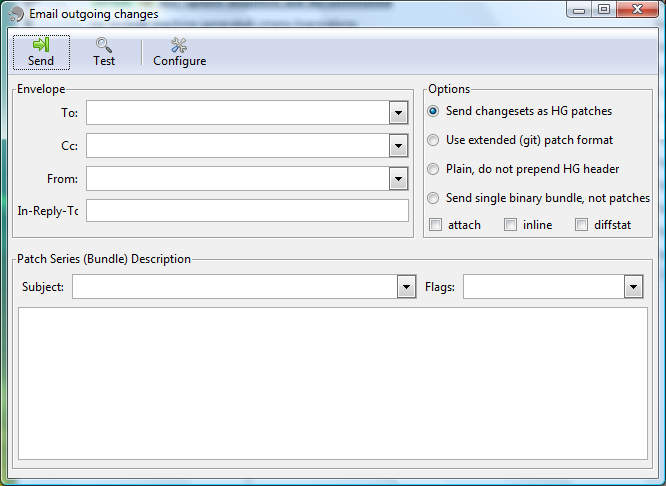
\includegraphics{email.png}
\caption{Email dialog of Repository Explorer}\end{figure}

To send a changeset as an email, use the changeset context menu of the
Repository Explorer. \emph{Export \(\rightarrow\) Email Patch}.  This
opens the e-mail dialog for this single changeset.

To send a changeset range, use the changeset range selection feature of
the Repository Explorer and select
\emph{Email from here to selected...}

Lastly, you can use the \textbf{Email} button on the syncbar of the
Repository Explorer to email all outgoing changes to the selected remote
repository.

\begin{notice}{note}{Note:}
You must configure
\href{http://www.selenic.com/mercurial/hgrc.5.html\#smtp}{SMTP}
to send patches via email
\end{notice}


\subsection{Cherry Picking}

Use the changeset range selection feature of the Repository Explorer and
select \emph{Diff with selected}.  This opens up a status
viewer showing you the accumulated changes between your base and target
changesets.

From the status viewer, you can select files and diff hunks just as you
can in the commit tool, and preview the final result in the
\textbf{Save Preview} tab.  Pressing \textbf{Save As} will save
the selected changes to a patch file.

For even finer cherry-picking, you can highlight a number of diff-hunks
in the hunk selection pane and hit CTRL-C.  This will copy the
highlighted (mouse selected, not toggled) hunks to the clipboard.

\begin{notice}{note}{Note:}
Reversing the order of your changeset selection reverses the effect
of the patch.
\end{notice}


\section{Import Patches}
\begin{figure}[htbp]
\centering

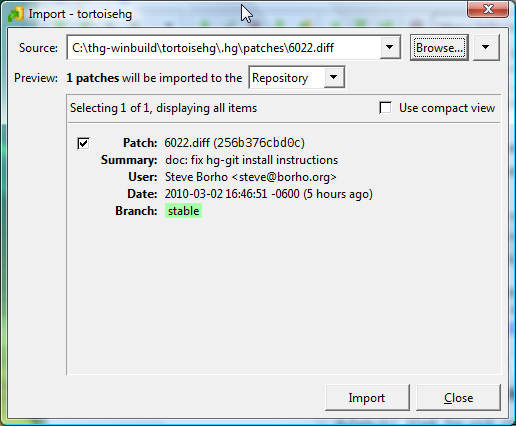
\includegraphics{import.png}
\caption{Import dialog of Repository Explorer}\end{figure}

The import dialog can be opened from the sync bar or menu of the
Repository Explorer, or via \textbf{hgtk import}.  The dialog supports
file and directory drag and drop.  The drop down menu in the upper right
corner next to the \textbf{Browse} button has the options:
\textbf{Browse Directory..} and \textbf{Import from Clipboard}.

You have the choice of importing directly into the repository, or
importing into your patch queue.

\begin{notice}{note}{Note:}
Importing a patch requires a clean working directory state.  You
must commit, revert, or shelve changes before importing a patch.
\end{notice}

\begin{notice}{warning}{Warning:}
If the patch you are importing does not have a commit
message, Mercurial will try to launch your editor, just as if you
had tried to import the patch from the command line.  Your ui.editor
needs to be a GUI app to make this work correctly.
\end{notice}


\section{Patch Queues}
\begin{figure}[htbp]
\centering

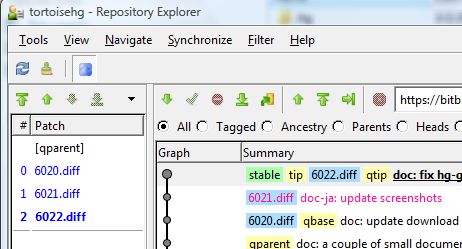
\includegraphics{patchqueue.png}
\caption{Patch Queue panel in the Repository Explorer}\end{figure}

Both the Repository Explorer and Commit Tool have an optional Patch
Queue panel that is only available when the user has enabled the MQ
extension.  It allows the user to perform most patch queue operations
including push, pop, rename, and finish.  It's recommended to learn the
MQ extension before using the Patch Queue panel.

\resetcurrentobjects
\hypertarget{--doc-extensions}{}

\chapter{Extensions}
\index{extensions (module)}
\hypertarget{module-extensions}{}
\declaremodule[extensions]{}{extensions}
\modulesynopsis{Describe extensions bundled with TortoiseHg binary packages}
This chapter describes Mercurial extensions that are shipped with
TortoiseHg binary packages for Windows.  These external extensions are
included as a convenience to users, so they can be easily enabled as
soon as they are needed.


\section{Hgfold}

\href{http://mercurial.selenic.com/wiki/CaseFoldExtension}{hgfold} is a
Mercurial extension that helps Windows users deal with filename case
collisions on VFAT and NTFS.

It adds options to the following Mercurial commands. Type
\textbf{hg help \textless{}command\textgreater{}} for more information:

\begin{Verbatim}[commandchars=@\[\]]
up    - allows you to update to a revision with filename collisions
merge - allows you to merge with a changeset that would create filename collisions
\end{Verbatim}

The extension does not currently do anything to prevent filename
collisions. See discussion on the Mercurial Wiki

\textbf{Installation}

To test the use of this plugin, you can specify it on the Mercurial
command line like this:

\begin{Verbatim}[commandchars=@\[\]]
hg --config "extensions.fold=" status
\end{Verbatim}

You may want to add it to your Mercurial.ini or a repository's hgrc like this:

\begin{Verbatim}[commandchars=@\[\]]
@PYGZlb[]extensions@PYGZrb[]
fold=
\end{Verbatim}

If you do this, you can omit the --config command-line option.

\textbf{Warnings}

Like all merge operations, fold.py has to change the parents of the
working directory. It is still in early testing, so use with caution.

If you get an error about an unknown changeset after running
\textbf{hg recover} try
\textbf{hg debugsetparents \textless{}number of tip revision\textgreater{}}.
You can find the number of the tip revision by running \textbf{hg log -l 2}.


\section{Hgcr-gui}

\href{http://bitbucket.org/glimchb/hgcr-gui/wiki/Home}{CodeReview} management tool
\begin{itemize}
\item {} 
This extension allows you to manage reviews for your code in any project you like.

\item {} 
It helps to keep the review management inside the mercurial.

\item {} 
One can add files to the review, remove them and notify reviewr that files are ready for review.

\item {} 
The reviewer can mark the code as `completed' review cycle and return the message to the developer.

\item {} 
The project manager can check the review status - which files are reviewd and which are not yet.

\item {} 
The extension will automatically spot the files that were changed since their last review and notify about that.

\item {} 
This extension uses GUI from TortoiseHg but also implements command line interface.

\item {} 
Code review database is stored in .code-review file in your repository root directory as a map of file and revision when review was done.

\end{itemize}

\textbf{Usage}:

\begin{Verbatim}[commandchars=@\[\]]
hg cr @PYGZlb[]OPTIONS@PYGZrb[] @PYGZlb[]FILES@PYGZrb[]

Code Review Plugin (requires Mercurial 1.3.x and TortoiseHg 0.9)

options:

 -c --complete  Mark CR as complete
 -a --add       Add files to CR list
 -r --remove    Remove files from CR list
 -l --list      Print files in CR list

use "hg -v help cr" to show global options
\end{Verbatim}

\begin{notice}{note}{Note:}
To start GUI don't give any options.
\end{notice}

\textbf{More Details}
\begin{itemize}
\item {} 
I've implemented the review around files and not changesets, because at the end,
I want to be able to tell for the specific project if all the files went through
code review process or not - the project status.

\item {} 
Suppose you have some project that you are in charge and many developers do
write code for it. And there is a group of reviewrs that review the developers code.

\item {} 
Is is very difficult to keep track of changes developers do, but simple to find
out what files have already been reviewd (by reviewers) and what were not.

\item {} 
Using this extension, Developer can mark his files (when finished development
process) as ``Ready for review'' and send notice to reviewer.

\item {} 
Reviewer will pick up the changeset (because changesets are stored in the code
review database) and perform code review (put notes inside the developer's code).

\item {} 
Afterwards Reviewr will mark the files as ``Review Completed'' and return the
notice to the developer.

\item {} 
The project manager can follow every time what is going on with his/her project.

\end{itemize}

\textbf{Installation}

You may want to add it to your Mercurial.ini or a repository's hgrc like this:

\begin{Verbatim}[commandchars=@\[\]]
@PYGZlb[]extensions@PYGZrb[]
hgcr-gui=
\end{Verbatim}


\section{Perfarce}

\href{http://www.kingswood-consulting.co.uk/hg/perfarce/}{Perfarce} home
page.

This extension is documented elsewhere.


\section{HGEOL}

The hgeol extension is the eventual successor to the win32text
extension.  It tries to resolve the EOLN compatibility problems in a
more complete and robust fashion.  Instead of documenting it here, we
will link to it's online documents which are continually evolving.
\begin{itemize}
\item {} 
\href{http://mercurial.selenic.com/wiki/EOLTranslationPlan}{EOLTranslationPlan}

\item {} 
\href{http://bitbucket.org/mg/hg-eol/}{Source code}

\end{itemize}


\section{Mercurial-Keyring}
\begin{itemize}
\item {} 
\href{http://pypi.python.org/pypi/mercurial\_keyring}{Mercurial Keyring} home page

\item {} 
\href{http://mercurial.selenic.com/wiki/KeyringExtension}{Keyring Extension} wiki page

\end{itemize}

Keyring extension uses services of the keyring library to securely save
authentication passwords (HTTP/HTTPS and SMTP) using system specific
password database (Gnome Keyring, KDE KWallet, OSXKeyChain, dedicated
solutions for Win32 and command line).

\textbf{What it does}

The extension prompts for the HTTP password on the first pull/push
to/from given remote repository (just like it is done by default), but
saves the password (keyed by the combination of username and remote
repository url) in the password database. On the next run it checks for
the username in .hg/hgrc, then for suitable password in the password
database, and uses those credentials if found.

Similarly, while sending emails via SMTP server which requires
authorization, it prompts for the password on first use of given server,
then saves it in the password database and reuses on successive runs.

In case password turns out incorrect (either because it was invalid, or
because it was changed on the server) it just prompts the user again.

\textbf{Installation}

First, the extension must be enabled in your Mercurial.ini file as:

\begin{Verbatim}[commandchars=@\[\]]
@PYGZlb[]extensions@PYGZrb[]
mercurial@_keyring=
\end{Verbatim}

\textbf{Password backend configuration}

The most appropriate password backend should usually be picked automatically,
without configuration. Still, if necessary, it can be configured using
\textasciitilde{}/keyringrc.cfg file (keyringrc.cfg in the home directory of the current user).
Refer to \href{http://pypi.python.org/pypi/keyring}{keyring docs}
for more details.

\begin{notice}{note}{Note:}
On Windows XP and above, your encrypted passwords are stored in the
credentials subsystem using
\href{http://msdn.microsoft.com/en-us/library/aa374804\%28VS.85\%29.aspx}{CredRead} and \href{http://msdn.microsoft.com/en-us/library/aa375187\%28VS.85\%29.aspx}{CredWrite}
\end{notice}

\begin{notice}{note}{Note:}
On Windows 2K, the encrypted passwords are stored in the system
registry under HKCU\textbackslash{}Software\textbackslash{}Mercurial\textbackslash{}Keyring.
\end{notice}

\textbf{Repository configuration (HTTP)}

Edit repository-local .hg/hgrc and save there the remote repository path and
the username, but do not save the password. For example:

\begin{Verbatim}[commandchars=@\[\]]
@PYGZlb[]paths@PYGZrb[]
myremote = https://my.server.com/hgrepo/someproject

@PYGZlb[]auth@PYGZrb[]
myremote.schemes = http https
myremote.prefix = my.server.com/hgrepo
myremote.username = mekk
\end{Verbatim}

Simpler form with url-embedded name can also be used:

\begin{Verbatim}[commandchars=@\[\]]
@PYGZlb[]paths@PYGZrb[]
bitbucket = https://User@PYGZat[]bitbucket.org/User/project@_name/
\end{Verbatim}

\begin{notice}{note}{Note:}
If both username and password are given in .hg/hgrc, extension will
use them without using the password database. If username is not
given, extension will prompt for credentials every time, also
without saving the password. So, in both cases, it is effectively
reverting to the default behaviour.
\end{notice}

Consult \href{http://www.selenic.com/mercurial/hgrc.5.html\#auth}{{[}auth{]}}
section documentation for more details.

\textbf{Repository configuration (SMTP)}

Edit either repository-local .hg/hgrc, or \textasciitilde{}/.hgrc (the latter is usually
preferable) and set there all standard email and smtp properties, including
smtp username, but without smtp password. For example:

\begin{Verbatim}[commandchars=@\[\]]
@PYGZlb[]email@PYGZrb[]
method = smtp
from = Joe Doe @textless[]Joe.Doe@PYGZat[]remote.com@textgreater[]

@PYGZlb[]smtp@PYGZrb[]
host = smtp.gmail.com
port = 587
username = JoeDoe@PYGZat[]gmail.com
tls = true
\end{Verbatim}

Just as in case of HTTP, you must set username, but must not set password here
to use the extension, in other cases it will revert to the default behaviour.

\textbf{Usage}

Configure the repository as above, then just pull and push (or email) You
should be asked for the password only once (per every username +
remote\_repository\_url combination).

\resetcurrentobjects
\hypertarget{--doc-nonhg}{}

\chapter{Use with other VCS systems}
\index{nonhg (module)}
\hypertarget{module-nonhg}{}
\declaremodule[nonhg]{}{nonhg}
\modulesynopsis{Describe using TortoiseHg as a front-end to other VCS}
This chapter describes the three most popular Mercurial extensions for
interoperating with \emph{foreign} VCS systems.  See also \href{http://mercurial.selenic.com/wiki/RepositoryConversion}{Repository
Conversion}


\section{Perfarce (Perforce)}
\begin{itemize}
\item {} 
\href{http://www.kingswood-consulting.co.uk/hg/perfarce/}{Perfarce} home page.

\item {} 
\href{http://mercurial.selenic.com/wiki/PerforceConcepts}{Mercurial for Perforce users}

\end{itemize}

This extension modifies the remote repository handling so that repository
paths that resemble:

\begin{Verbatim}[commandchars=@\[\]]
p4://p4server@PYGZlb[]:port@PYGZrb[]/clientname
\end{Verbatim}

cause operations on the named p4 client specification on the p4 server.
The client specification must already exist on the server before using
this extension. Making changes to the client specification Views causes
problems when synchronizing the repositories, and should be avoided.

Five built-in Mercurial commands are overridden.

outgoing:

\begin{Verbatim}[commandchars=@\[\]]
If the destination repository name starts with p4:// then this
reports files affected by the revision(s) that are in the local
repository but not in the p4 depot.
\end{Verbatim}

push:

\begin{Verbatim}[commandchars=@\[\]]
If the destination repository name starts with p4:// then this
exports changes from the local repository to the p4 depot. If no
revision is specified then all changes since the last p4 changelist
are pushed. In either case, all revisions to be pushed are foled
into a single p4 changelist.  Optionally the resulting changelist is
submitted to the p4 server, controlled by the --submit option to
push, or by setting **perfarce.submit** to True.  If the option
**perfarce.keep** is False then after a successful submit the files
in the p4 workarea will be deleted.
\end{Verbatim}

pull:

\begin{Verbatim}[commandchars=@\[\]]
If the source repository name starts with p4:// then this imports
changes from the p4 depot, automatically creating merges of
changelists submitted by hg push.  If the config option
**perfarce.keep** is False then the import does not leave files in
the p4 workarea, otherwise the p4 workarea will be updated with the
new files.
\end{Verbatim}

incoming:

\begin{Verbatim}[commandchars=@\[\]]
If the source repository name starts with p4:// then this
reports changes in the p4 depot that are not yet in the local
repository.
\end{Verbatim}

clone:

\begin{Verbatim}[commandchars=@\[\]]
If the source repository name starts with p4:// then this
creates the destination repository and pulls all changes from
the p4 depot into it.
\end{Verbatim}

\emph{TortoiseHg Integration}

When the perfarce extension is enabled, it adds a \textbf{start revision}
configurable option to the clone tool, and a \textbf{Perforce} menu
to the Repository Explorer.  The menu has two items:

identity:

\begin{Verbatim}[commandchars=@\[\]]
Finds the tip Perforce changelist in your local repository and
selects it in the changelog window.
\end{Verbatim}

pending:

\begin{Verbatim}[commandchars=@\[\]]
Detects pending Perforce changelists that have been "push"ed to your
Perforce client but have not been submitted, or have not been pulled
back.  This opens the pending changelist dialog so that you can view
these pending changelists and either submit or revert them.
\end{Verbatim}

\emph{Installation}

Perfarce comes bundled with TortoiseHg 1.0 Windows installers, so you
enable perfarce by simply adding it to your Mercurial.ini or a
repository's hgrc like this:

\begin{Verbatim}[commandchars=@\[\]]
@PYGZlb[]extensions@PYGZrb[]
perfarce=
\end{Verbatim}


\section{hgsubversion (SVN)}
\begin{itemize}
\item {} 
\href{http://bitbucket.org/durin42/hgsubversion/wiki/Home}{hgsubversion} home page

\item {} 
\href{http://mercurial.selenic.com/wiki/HgSubversion}{hgsubversion Extension} wiki page

\item {} 
\href{http://mercurial.selenic.com/wiki/WorkingWithSubversion}{Working with Subversion Repositories}

\end{itemize}

hgsubversion, as it's name implies, allows you to use Mercurial as a
client to a Subversion server.  It can also be used to do straight
conversions of Subversion repositories into Mercurial.

\emph{Installation}

TortoiseHg Windows installers come with the python-svn bindings that
hgsubversion requires, so one only needs to clone the hgsubversion
repository to your local computer:

\begin{Verbatim}[commandchars=@\[\]]
hg clone http://bitbucket.org/durin42/hgsubversion/ C:\hgsvn
\end{Verbatim}

Then enable the extension in your Mercurial.ini file, specifying the
hgsubversion folder inside the cloned repository:

\begin{Verbatim}[commandchars=@\[\]]
@PYGZlb[]extensions@PYGZrb[]
hgsubversion = C:\hgsvn\hgsubversion
\end{Verbatim}

You can verify that worked by typing \textbf{hg help hgsubversion}

See the hgsubversion wiki for details of use.

\begin{notice}{warning}{Warning:}
When doing a clone of a Subversion server, it is highly recommended
to clone only the first few revisions, then pull the rest.  Clone's
failure behavior is to delete the entire incomplete cloned
repository.  Pull is much more forgiving.
\end{notice}

\emph{TortoiseHg Integration}

Imported Subversion changesets will display the original Subversion
checkin number in the Repository Explorer browser.


\section{hg-git (git)}
\begin{itemize}
\item {} 
\href{http://hg-git.github.com/}{hg-git} home page

\item {} 
\href{http://mercurial.selenic.com/wiki/HgGit}{hg-git Extension} wiki page

\item {} 
\href{http://mercurial.selenic.com/wiki/GitConcepts}{Mercurial for Git users}

\end{itemize}

hg-git, as it's name implies, allows you to use Mercurial as a
client to a git server.  It can also be used to do straight conversions
of Git repositories into Mercurial.

\emph{Installation}

TortoiseHg Windows installers come with the python-git bindings (named
dulwich) that hg-git requires, so one only needs to clone the
hg-git repository to your local computer:

\begin{Verbatim}[commandchars=@\[\]]
hg clone http://bitbucket.org/durin42/hg-git/ C:\hg-git
\end{Verbatim}

Then enable hggit and bookmarks in your Mercurial.ini file:

\begin{Verbatim}[commandchars=@\[\]]
@PYGZlb[]extensions@PYGZrb[]
bookmarks =
hggit = C:\hg-git\hggit
\end{Verbatim}

You can verify that worked by typing \textbf{hg help hggit}

See the hggit documentation for details of use.

Beware the `incoming' command appears broken when speaking with git
repositories, and `outgoing' does not show much useful info. So you are
restricted to simple push and pull commands (not uncommon for extensions
that speak with external revision control tools).

\resetcurrentobjects
\hypertarget{--doc-faq}{}

\chapter{Frequently Asked Questions}

\emph{What is TortoiseHg?}
\begin{quote}

A Windows shell extension for the Mercurial revision control system,
similar to the Tortoise clients for Subversion and CVS. It also
includes an hgtk application for command line use on many platforms.
\end{quote}

\emph{What comes included in the TortoiseHg binary installer for Windows?}
\begin{quote}

\href{http://mercurial.selenic.com/wiki/}{Mercurial},
\href{http://kdiff3.sourceforge.net/}{kdiff3},
\href{http://www.chiark.greenend.org.uk/\%7Esgtatham/putty/}{TortoisePlink}
five bonus extensions: hgfold, hgcr-gui, perfarce, hgeol, mercurial-keyring.
python-svn for hgsubversion and convert extensions
dulwich for hg-git use.
See \code{extension-versions.txt} in installer root for more details
\end{quote}

\emph{Is Mercurial on Windows compatible with the index service and virus scanners?}
\begin{quote}

No. Like TortoiseSVN, \href{http://www.selenic.com/pipermail/mercurial/2010-January/029680.html}{we recommend}
to turn off the indexing service on the working copies and repositories,
and exclude them from virus scans.
\end{quote}

\emph{How can I get translations for the Explorer context menu?}
\begin{quote}

The available translations were stored by the installer under
\code{C:\textbackslash{}Program Files\textbackslash{}TortoiseHg\textbackslash{}i18n\textbackslash{}cmenu}.  Select the
locale you would like to use, double-click on it, and confirm all
requests.
\end{quote}

\emph{Can I configure the toolbars in TortoiseHg applications?}
\begin{quote}

TortoiseHg dialogs are PyGtk applications, so they can be configured by
modifying the gtkrc file that is installed as
\code{C:\textbackslash{}Program Files\textbackslash{}TortoiseHg\textbackslash{}gtk\textbackslash{}etc\textbackslash{}gtk-2.0\textbackslash{}gtkrc}:

\begin{Verbatim}[commandchars=@\[\]]
gtk@PYGbe[-]toolbar@PYGbe[-]icon@PYGbe[-]size @PYGbe[=] GTK@_ICON@_SIZE@_LARGE@_TOOLBAR
@PYGaE[@# Pick an icon size from:]
@PYGaE[@# GTK@_ICON@_SIZE@_MENU]
@PYGaE[@# GTK@_ICON@_SIZE@_SMALL@_TOOLBAR]
@PYGaE[@# GTK@_ICON@_SIZE@_LARGE@_TOOLBAR   (default)]
@PYGaE[@# GTK@_ICON@_SIZE@_BUTTON]
@PYGaE[@# GTK@_ICON@_SIZE@_DND]
@PYGaE[@# GTK@_ICON@_SIZE@_DIALOG]
gtk@PYGbe[-]toolbar@PYGbe[-]style @PYGbe[=] GTK@_TOOLBAR@_BOTH
@PYGaE[@# Pick a toolbar style from:]
@PYGaE[@# GTK@_TOOLBAR@_ICONS]
@PYGaE[@# GTK@_TOOLBAR@_TEXT]
@PYGaE[@# GTK@_TOOLBAR@_BOTH              (default)]
@PYGaE[@# GTK@_TOOLBAR@_BOTH@_HORIZ]
\end{Verbatim}

These settings are applied globally to all TortoiseHg applications.
\end{quote}

\emph{How do I do merges and arbitrary version checkouts?}
\begin{quote}

Merges and updates are intended to be done from within the Changelog
tool (\textbf{Repository Explorer} menu option)
\end{quote}

\emph{How do I use TortoiseHg's shelve extension from the hg command line?}
\begin{quote}

Enable the extension in your Mercurial.ini file:

\begin{Verbatim}[commandchars=@\[\]]
@PYGZlb[]extensions@PYGZrb[]
tortoisehg.util.hgshelve=
\end{Verbatim}
\end{quote}

\emph{Why can't I connect to an ssh server (TortoisePlink.exe} \code{...cannot execute specified...} \emph{error message)?}
\begin{quote}

See \href{http://bitbucket.org/tortoisehg/stable/wiki/ssh}{ssh}.
\end{quote}

\emph{Why can't I connect to an ssh server (remote: bash: \textless{}server name\textgreater{}: command not found)?}
\begin{quote}

TortoisePlink (and basic Plink) will try to use the \textbf{Host
Name} configured in Putty under the \textbf{Default Settings}.
It adds this host name to its command line parameters, causing the
hostname to be specified twice, causing this particular error.
Clearing the host name from the \textbf{Default Settings} is a
possible workaround.
\end{quote}

\emph{How can I use tool X as my visual diff tool?}
\begin{quote}

Since version 1.0, TortoiseHg should autodetect most popular visual
diff tools and make them available for selection from the
\textbf{Visual Diff Tool} item in the settings tool.
\end{quote}

\emph{I'm a CLI user, how do I disable the shell extension (overlay icons and context menus)?}
\begin{quote}

Simply ask the installer to remove the shell extension entirely.
\end{quote}

\emph{How is TortoiseHg configured?}
\begin{quote}

TortoiseHg gets configuration settings from two systems.
\begin{enumerate}
\item {} \begin{description}
\item[The Mercurial configuration system, which is three-tiered]\begin{enumerate}
\item {} 
Site-wide \code{Mercurial.ini} in \code{\%ProgramFiles\%\textbackslash{}TortoiseHg}

\item {} 
Per-User \code{Mercurial.ini} in \code{\%UserProfile\%}

\item {} 
Per-Repository \code{Mercurial.ini} in \code{repo-root\textbackslash{}.hg\textbackslash{}hgrc}

\end{enumerate}

\end{description}

\item {} 
\code{\%APPDATA\%\textbackslash{}Tortoisehg} settings for application state
(window positions, etc)

\end{enumerate}

These are some of the configurables that are stored the Mercurial
configuration system.

\begin{Verbatim}[commandchars=@\[\]]
@PYGZlb[]tortoisehg@PYGZrb[]
vdiff @PYGbe[=] vdiff
editor @PYGbe[=] gvim
tabwidth @PYGbe[=] @PYGaw[4]
longsummary @PYGbe[=] @PYGaA[True]
graphlimit @PYGbe[=] @PYGaw[500]
authorcolor @PYGbe[=] @PYGaA[True]
authorcolor@PYGbe[.]steve @PYGbe[=] blue
\end{Verbatim}
\end{quote}

\emph{Is it possible to change fonts?}
\begin{quote}

In some cases, yes. The gtools based dialogs (commit, status,
shelve) allow some font configuration.

\begin{Verbatim}[commandchars=@\[\]]
@PYGZlb[]gtools@PYGZrb[]
@# font used in changeset viewer and commit log text
fontcomment = courier 10
@# font used for diffs in status and commit tools
fontdiff = courier 10
@# font used in file lists in status and commit tools
fontlist = courier 9
@# font used in command output window
fontlog = courier 10
\end{Verbatim}
\end{quote}

\emph{How do I switch GTK themes?}
\begin{quote}

You also should be able to download new themes and copy them into
the \code{gtk\textbackslash{}share\textbackslash{}themes} directory and then enable them in
\code{gtk\textbackslash{}etc\textbackslash{}gtk-2.0\textbackslash{}gtkrc}.
\end{quote}

\emph{Where do TortoiseHg extensions look for external Python modules on Windows?}
\begin{quote}

TortoiseHg includes an entire Python distribution bundled up as
DLLs. The standard library modules are all in the
\code{library.zip} file in \code{C:\textbackslash{}Program Files\textbackslash{}TortoiseHg}.

If you try to use an extension that imports a non-standard Python
module, you will find that the extension will fail to load because
it can't find the module. For example the ReviewBoard extension
imports the simplejson module, which is not part of the standard
Python distribution.

In order to make it work you need to add a couple of lines to the
top of the extension's .py file, before the line that imports the
foreign module:

\begin{Verbatim}[commandchars=@\[\]]
@PYGal[import] @PYGaW[sys]
sys@PYGbe[.]path@PYGbe[.]append(@PYGaB[r']@PYGaB[C:]@PYGaB[\]@PYGaB[path]@PYGaB[\]@PYGaB[to]@PYGaB[\]@PYGaB[module]@PYGaB['])
\end{Verbatim}

Note that this will not work for modules distributed as .egg files;
the supplied path must contain the module's .py or .pyc files.

If you have many extensions and/or hooks that all share the same
Python package, you can create an extension which explicitly
modifies sys.path for all the others.  Simply name the extension
such that it is loaded first (alphabetically).  Something like:

\begin{Verbatim}[commandchars=@\[\]]
@PYGZlb[]extensions@PYGZrb[]
00setSysPath = C:\path\to\setsyspath.py
\end{Verbatim}
\end{quote}

\emph{How do I fix odd characters in dialog?}
\begin{quote}

Since 0.8, we no longer distribute multiple themes and switched
default theme to MS-Windows.  As a result, it might causes an issue
related default font of MS-Windows theme in some environments.  In
order to fix this issue, add following setting to TortoiseHg's
\code{gtkrc} file:

\begin{Verbatim}[commandchars=@\[\]]
style "msw-default"
{
font@_name = "MS UI Gothic 9"
}
\end{Verbatim}

You can find \code{gtkrc} file in your TortoiseHg install directory:
i.e. \code{C:\textbackslash{}Program Files\textbackslash{}TortoiseHg\textbackslash{}gtk\textbackslash{}etc\textbackslash{}gtk-2.0\textbackslash{}gtkrc}
\end{quote}

\resetcurrentobjects
\hypertarget{--doc-debugging}{}

\chapter{Debugging}
\index{debugging (module)}
\hypertarget{module-debugging}{}
\declaremodule[debugging]{}{debugging}
\modulesynopsis{Debug problems in shell extension or dialogs}

\section{Dialogs}

Stderr is being captured to a buffer that is being inspected at program
exit.  If any serious errors (tracebacks, etc) are found in the stderr
buffer the entire contents are sent to the bug report tool so the user
can (should) report a bug.  If you suspect there are errors that are not
being reported, you can set the environment variable \textbf{THGDEBUG} to any
value to disable the stderr buffering.

If you have a bit of Python knowledge, you can also use:

\begin{Verbatim}[commandchars=@\[\]]
hgtk --debugger @textless[]command@textgreater[]
\end{Verbatim}

To disable the forking behavior of hgtk, you can either set an
environment variable \textbf{THG\_HGTK\_SPAWN}, or add the command line
parameter `--nofork'.


\subsection{Windows}

To debug the changelog viewer, for instance, enter these commands
into a \textbf{cmd.exe} window, while inside the repository:

\begin{Verbatim}[commandchars=@\[\]]
set THGDEBUG=1
hgtk log
\end{Verbatim}


\subsection{Linux/MacOSX}

To debug the changelog viewer, for instance, enter these commands
into your shell window, while inside the repository:

\begin{Verbatim}[commandchars=@\[\]]
export THGDEBUG=1
hgtk log
\end{Verbatim}


\section{Shell Extension}

The debugging mechanisms depend on your platform.


\subsection{Windows}

See also \href{http://msdn.microsoft.com/en-us/library/cc144064(VS.85).aspx}{http://msdn.microsoft.com/en-us/library/cc144064(VS.85).aspx}
for some info bits about Running and Testing Shell Extensions on Windows

The \textbf{DbgView} tool from the SysInternals suite will capture
debug messages from the shell extension.  However, the shell
extension does not emit debugging info by default.  It must be enabled
by setting the registry key defined in
\code{win32/shellext/DebugShellExt.reg} in the TortoiseHg source
repository.  You can double-click on this file to load the key into your
registry.

Another option is to exit the \textbf{ThgTaskbar} system tray
application and start it from the command line.  It will emit some debug
information to the console.


\subsection{Nautilus}

Debugging is done via the environment variable DEBUG\_THG
\begin{itemize}
\item {} 
to test in a separate process:

\begin{Verbatim}[commandchars=@\[\]]
DEBUG@_THG=Ne TMPDIR=/tmp/anydir/ --no-desktop nautilus @PYGZlb[]path@PYGZrb[]
\end{Verbatim}

\item {} 
to test in the main instance:

\begin{Verbatim}[commandchars=@\[\]]
nautilus -q
DEBUG@_THG=NOe nautilus
\end{Verbatim}

\item {} 
permanent debugging, set DEBUG\_THG in a file which is read on session
start (\textasciitilde{}/.profile, \textasciitilde{}/.xprofile)

\end{itemize}

Upper case characters in DEBUG\_THG specify modules.  Only \emph{O} and \emph{N}
for \emph{OverlayCache} and \emph{Nautilus}, respectively, are supported module
names.  Lower case characters imply parts. Only \emph{e} is supported,
implying \emph{error} messages.

To restart nautilus, chose either
\begin{enumerate}
\item {} 
killall nautilus (the session restarts nautilus automatically, stdin and stdout go to \textasciitilde{}/.xsession-errors)

\item {} 
nautilus -q; nautilus (stdin and stdout are on the console)

\end{enumerate}


\chapter{Indices and tables}
\begin{itemize}
\item {} 
\emph{Index}

\item {} 
\emph{Module Index}

\item {} 
\emph{Search Page}

\end{itemize}


\renewcommand{\indexname}{Module Index}
\printmodindex
\renewcommand{\indexname}{Index}
\printindex
\end{document}
